%   preamble {{{1  %
%%%%%%%%%%%%%%%%%%%%

%\documentclass[notes=show]{beamer}
\documentclass[notes=hide]{beamer}

\usepackage[utf8]{inputenc}
\usepackage[english]{babel}
\usepackage[]{tikz}

\newcommand{\ket}[1]{\left| #1 \right>} % for Dirac bras
\newcommand{\bra}[1]{\left< #1 \right|} % for Dirac kets
\newcommand{\braket}[2]{\left< #1 \vphantom{#2} \right|\!\!
  \left. #2 \vphantom{#1} \right>} % for Dirac brackets

%  beamer theme {{{1  %
%%%%%%%%%%%%%%%%%%%%%%%

\usetheme{metropolis}           % Use metropolis theme
\metroset{background=light}
\setbeamertemplate{frame footer}{%

\includegraphics[width=1cm, keepaspectratio]{images/max_planck.png}
} %Metropolis defined
\setbeamercolor{background canvas}{bg=white}



\title[Ab initio studies \ldots]{%
  
\includegraphics[width=2cm, keepaspectratio]{images/max_planck.png}
 \hfill
  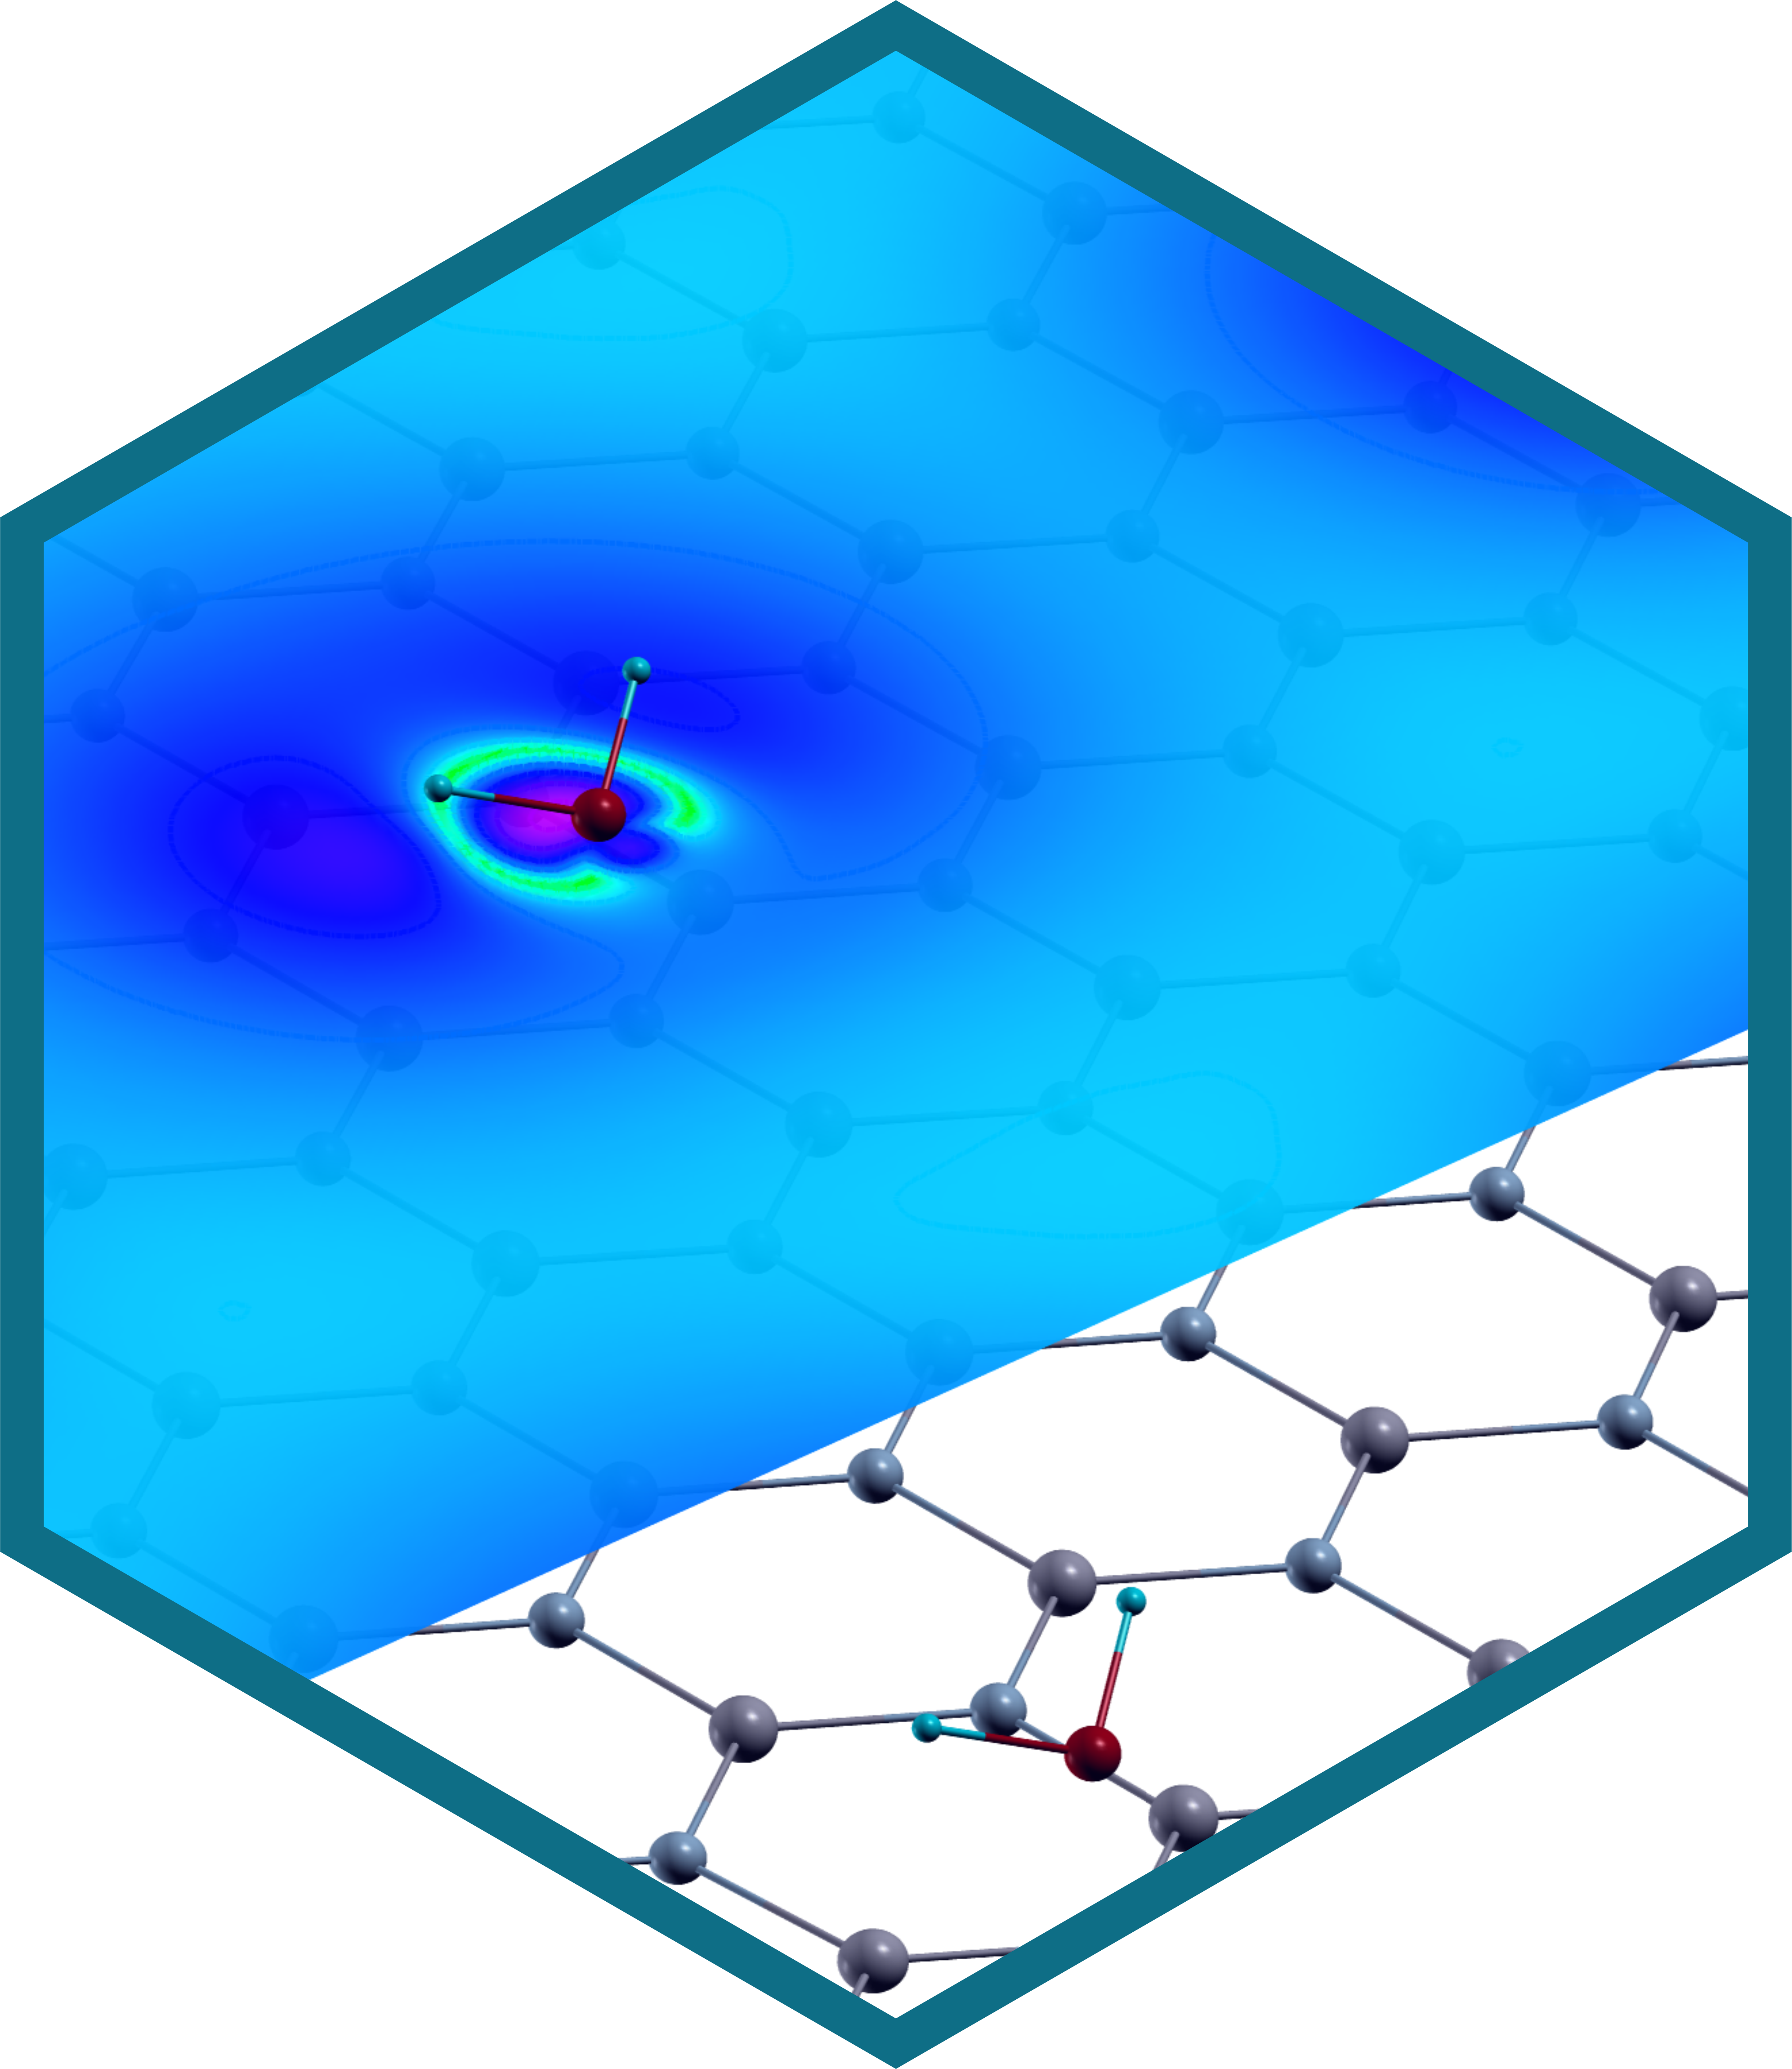
\includegraphics[width=1.4cm, keepaspectratio]{images/logo_andreas.png} \\
  Ab-initio studies of nitrogen-vacancy impurity complexes in diamond
}
\date{March 15, 2017}


\author{Alejandro Gallo}
\institute{%
  Max-Planck Institute for solid state research\\
  Stuttgart, Germany\\
  Prof.\ Andreas Gr\"uneis group\\
}


\begin{document}


%  title {{{1  %
%%%%%%%%%%%%%%%%

\maketitle

%\begin{frame}{Contents} %{{{1
  %\tableofcontents
%\end{frame}


%\section{Overview} %{{{1

\begin{frame}{Nitrogen Vacancy Centre in diamond (NV center)} %{{{1
  \begin{center}
    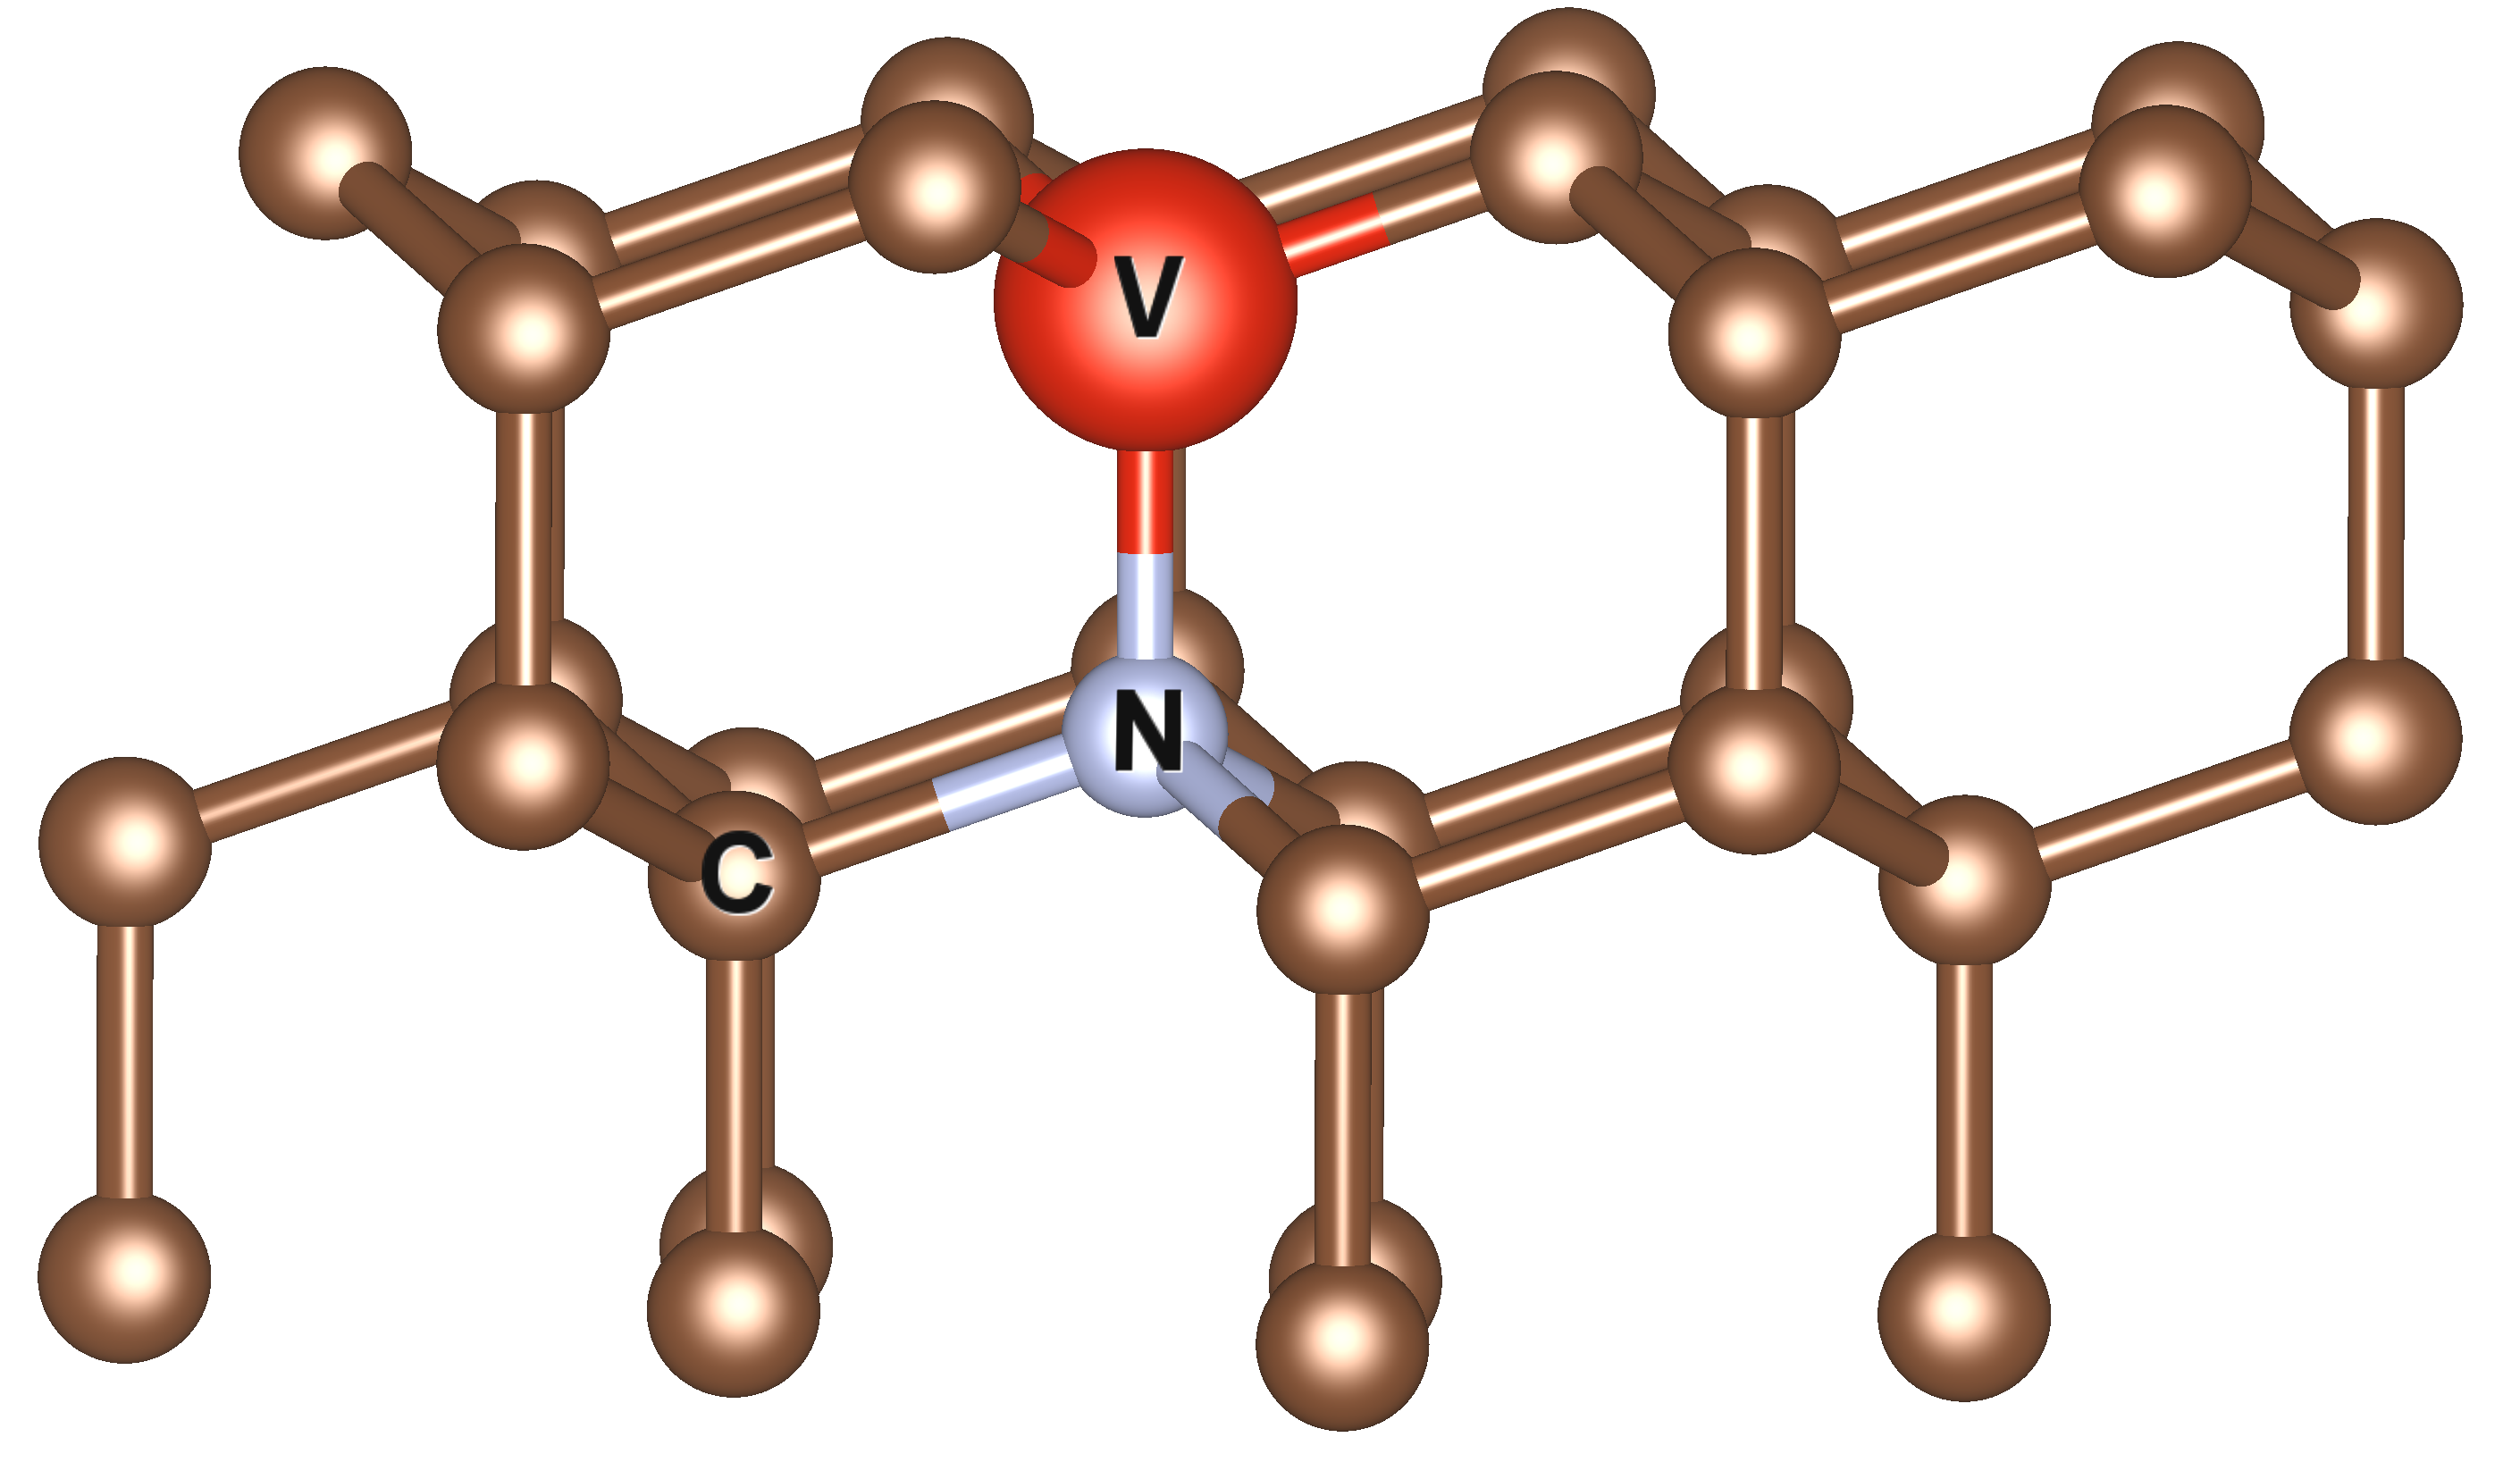
\includegraphics[width=0.9\textwidth]{images/POSCAR_16_view.png}
  \end{center}

  \note{

    So let us just begin by firstly introducing the main actor in this story.
    This is the Nitrogen vacancy impurity center in diamond, as most of you may
    already know.  The big red region is a vacant carbon site and next to it
    lies a nitrogen atom.

    This kind of defects has been researched now for almost 50 years.  However
    it was not until the late nineties when single negatively charged NV
    centres where found. This enabled the demonstration of photo stable single
    photon emitters, which is of course of huge importance for quantum optics.

    The most notable and studied of the NV centers is the negatively charged
    one.

  }

\end{frame}


\begin{frame}{Aims and motivation} %{{{1

  \begin{columns}
    \begin{column}{0.5\textwidth}
      \begin{itemize}

        \item
          Exploration of defect centres using state-of-the-art ab-initio
          theories.

        \item
          Systematic characterization of defect fingerprints.

        \item
          Search for new defects with tailored properties useful for practical
          applications.

        \item
          Benchmark ab-initio theories with well-known
          experimental data.


      \end{itemize}
    \end{column}
    \begin{column}{0.5\textwidth}
      \begin{center}
        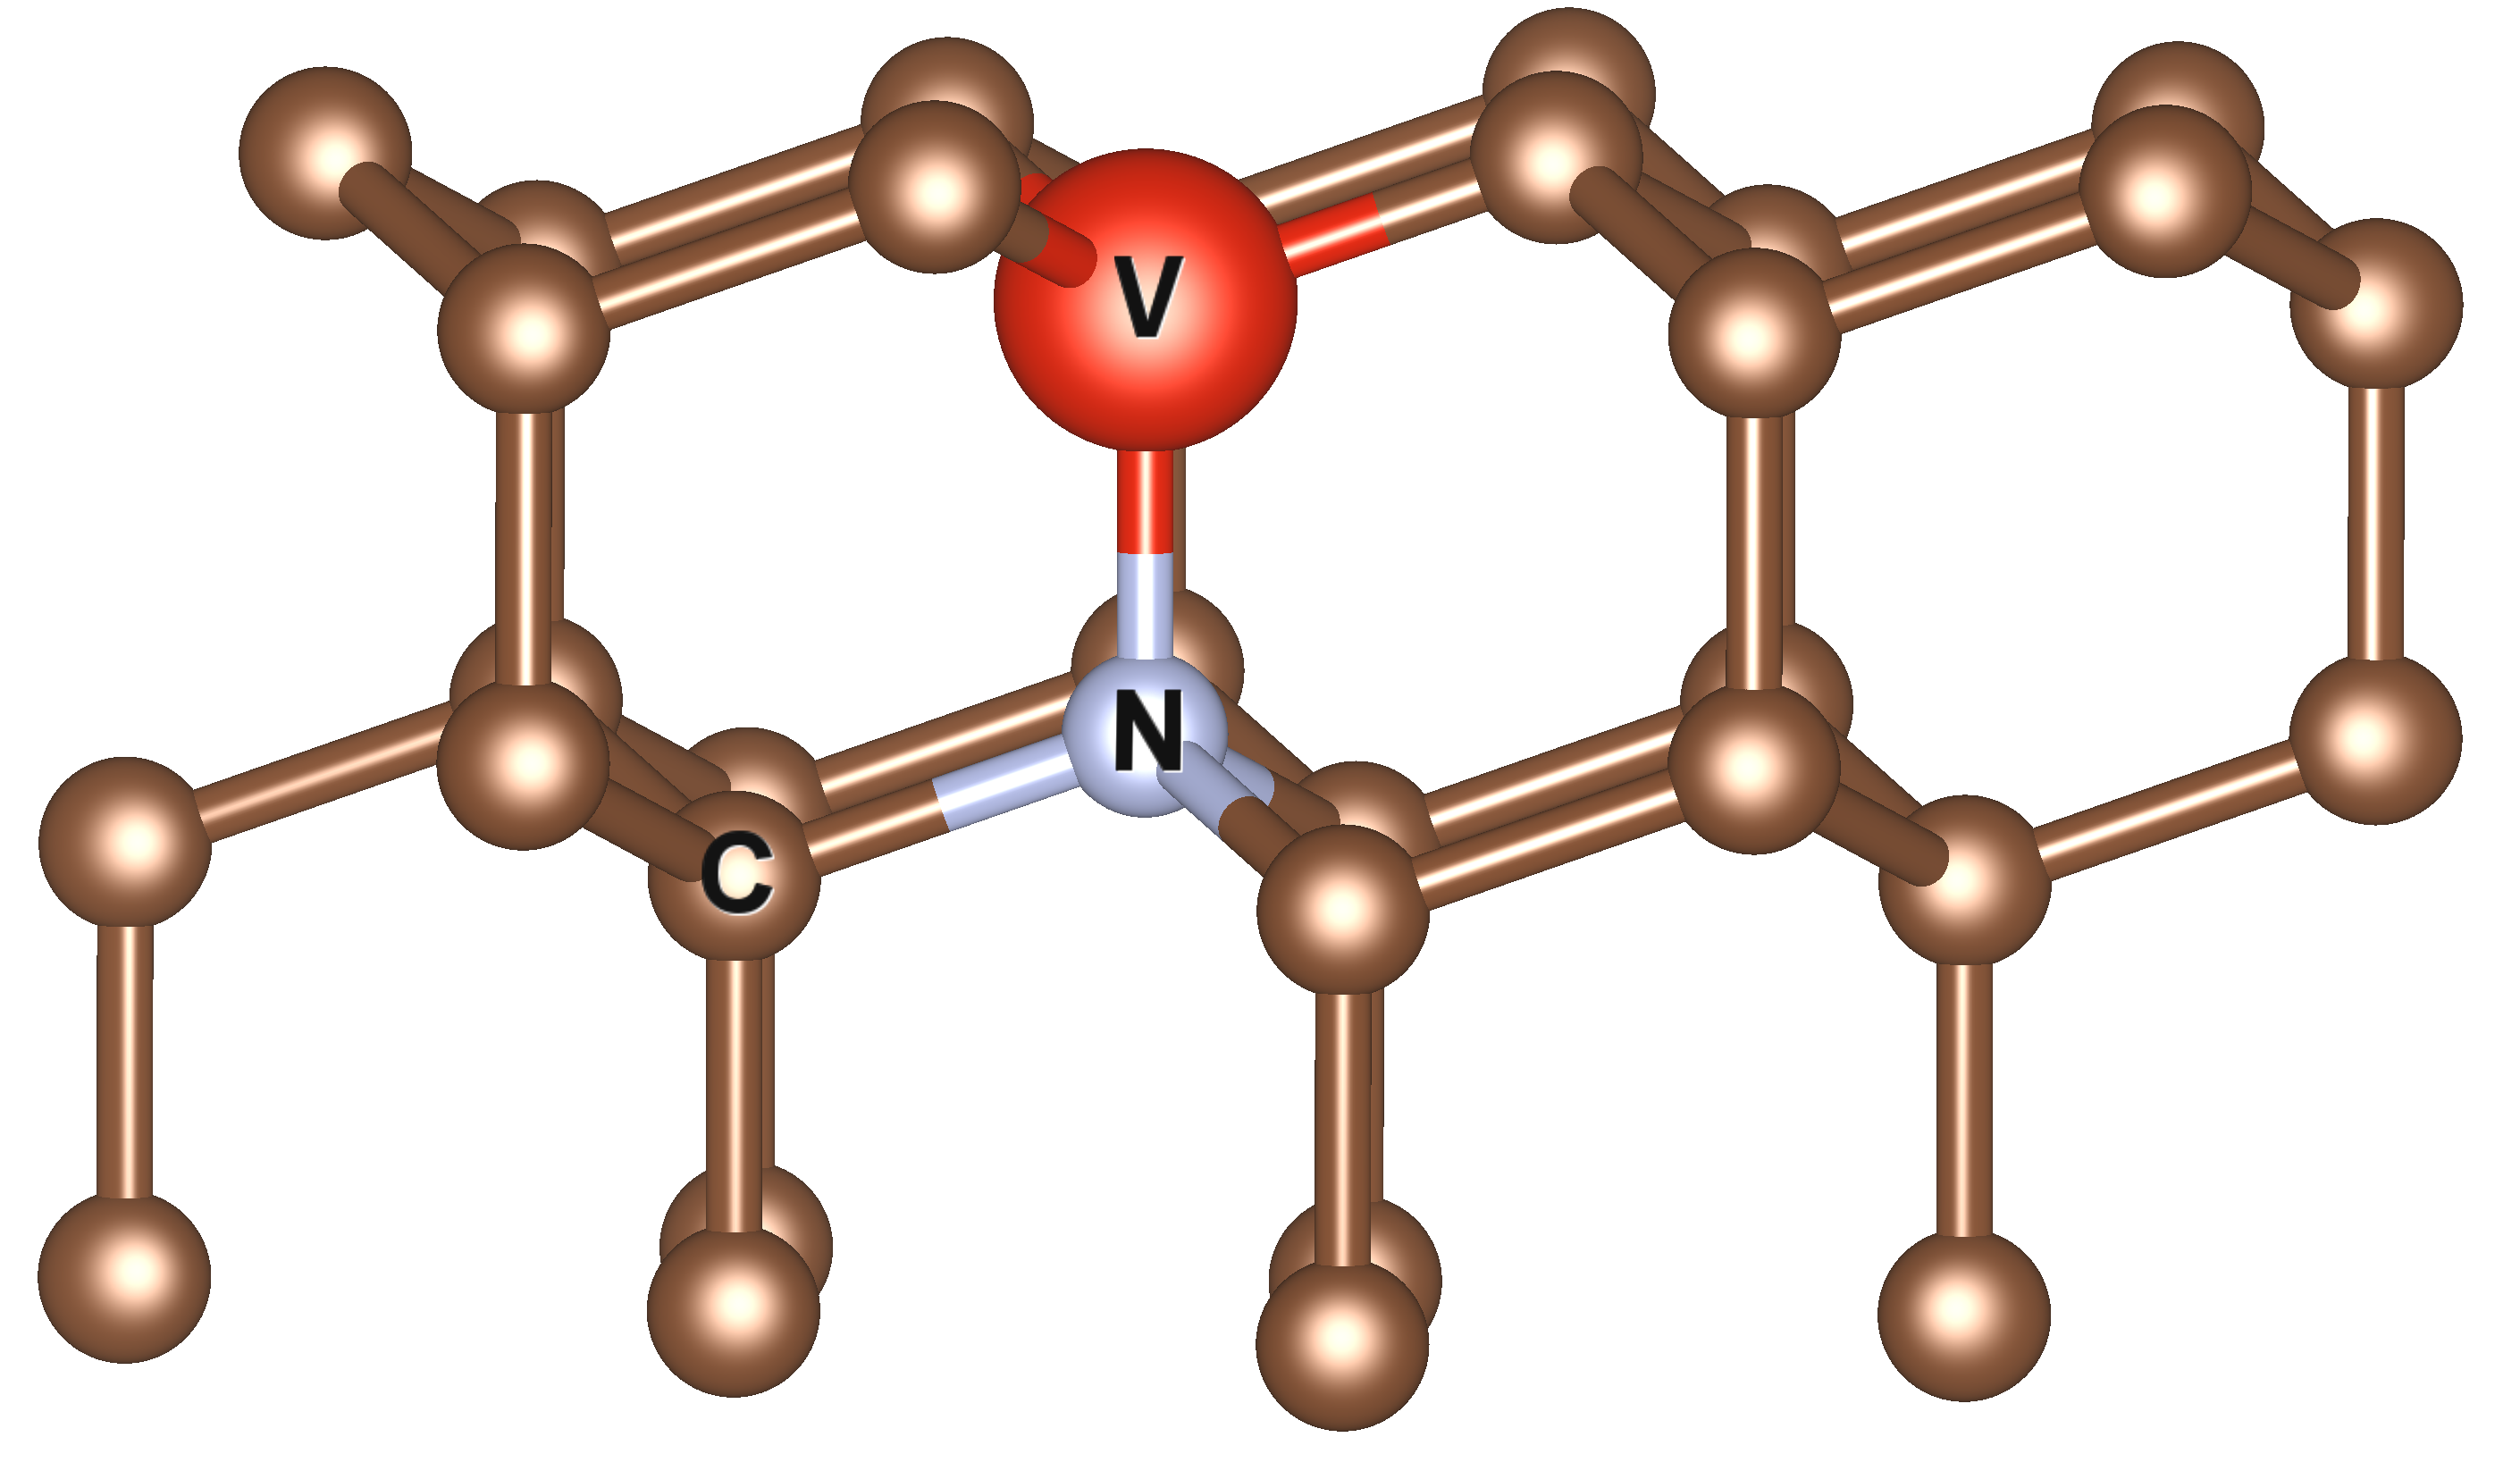
\includegraphics[width=1\textwidth]{images/POSCAR_16_view.png}
      \end{center}
    \end{column}
  \end{columns}

  \note{%

    So the main aim of this work is to computationally
    treat electronic properties of defect centers in diamond
    using state-of-the-art ab initio theories.

    Through this exploration we hope to recover many well-known
    experimentally verified quantities.

    In order to do this we use several purely theoretical
    results to orient our calculations into the right direction.
    (e.g. Markus' Gruppentheorierechnungen)

  }

\end{frame}



%\section{Introduction} %{{{1
%\begin{frame}{Ab initio} %{{{1
  \begin{center}
    Ab initio $ \equiv $ From first principles (only $ \hat{H} $)
  \end{center}
  \visible<2->{%
    \begin{center}
      Maxwell equations
      $ \Rightarrow $
      $ \mathbf{E}(x,y,z), \mathbf{B}(x,y,z) $
    \end{center}
  }
  \visible<3->{%
    \begin{center}
      $ \hat{H}_{N^{2}} $
      \visible<4->{%
        $ \Rightarrow  $
        7+7 $ e^{-} $
      }
      \visible<5->{%
        $ \Rightarrow  $
        $
        \Psi (\mathbf{r}_{1}, \ldots, \mathbf{r}_{14}) \quad \mathbf{r}_{i} =
        (x_{i}, y_{i}, z_{i})
        $, \\
      }
    \end{center}
    \visible<6->{%
      Store 4 points per coordinate (4-grid)
      $ \Rightarrow $
      \[
        4^{3\cdot 14}\ \mathrm{pts}
        \times
        \frac{64}{8}
        \frac{\mathrm{B}}{\mathrm{pts}}
        \times
        \frac{1}{2^{30}}
        \frac{\mathrm{GB}}{\mathrm{B}}
        \times
        \frac{1}{10}
        \frac{\mathrm{DVD}}{\mathrm{GB}}
        \times
        \frac{1}{10^{6}}
        \frac{\mathrm{km}}{\mathrm{DVD}}
        \approx
        288 L_{\mathrm{earth} - \mathrm{mars}}
      \]
    }
  }
\end{frame}

%\begin{frame}{Density functional theory (DFT)} %{{{1
  ``\textit{$ \Psi  $  contains too much information}''
  \hfill \textit{- Popular saying}
  \begin{itemize}
    \item In principle, DFT delivers the \textbf{exact ground state properties}.
    %\item The exact electronic ground state of a system is only dependent on
      %the electronic density $ \rho $ .

    \item All quantities are written in terms of $ \rho $ (functional formalism).
    \item E.g.:
      \begin{align*}
        &E[ \rho ] =\\
        &T_{s} [ \rho  ]
        +
        \int  V ( \mathbf{r} ) \rho ( \mathbf{r} ) \ \mathrm{d} \mathbf{r}
        +
        \frac{1}{4\pi \epsilon _{0}}
        \int
        \frac{\rho ( \mathbf{r} ) \rho ( \mathbf{r}' )}{| \mathbf{r} - \mathbf{r}'|}
        \ \mathrm{d} \mathbf{r}\mathrm{d} \mathbf{r}'
        +
        E^{\mathrm{exact}}_{\mathrm{xc}} [ \rho, \nabla \rho  ]
      \end{align*}
      The exchange correlation potential
      $ E^{ \mathrm{exact}}_{\mathrm{xc}} [\rho, \nabla\rho] $
      determines the DFT \textit{flavor}.
      In many calculations we use the so-called \textbf{PBE} \textit{(Perdew-Burke-Ernzerhof)} functional.
  \end{itemize}
\end{frame}


%\begin{frame}{Nitrogen Vacancy Center (Dangling bonds)} %{{{1
  \begin{columns}
    \begin{column}{0.5\textwidth}
      \begin{tikzpicture}
        \node at (0,0) {
            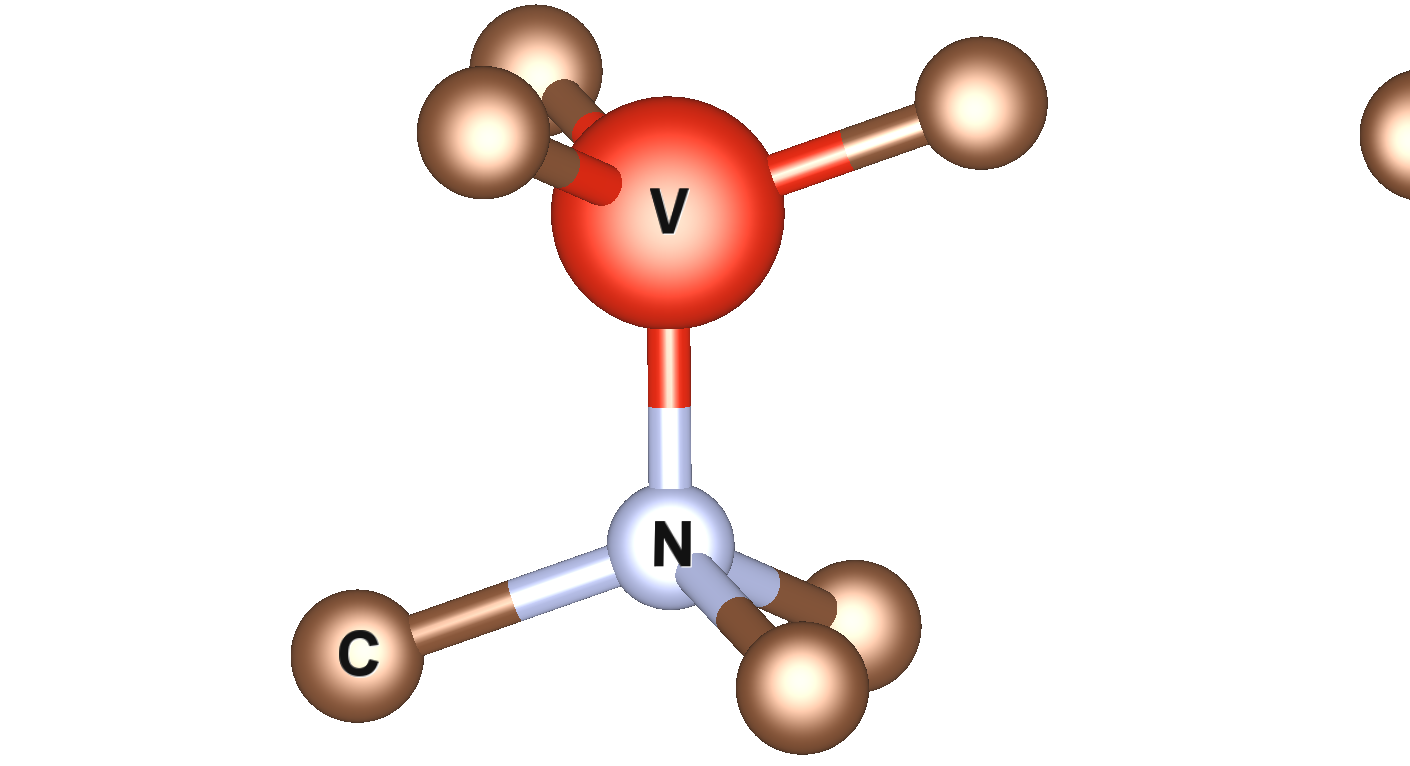
\includegraphics[clip, trim=9cm 0 12cm 0,width=1\textwidth]{images/POSCAR_16_view_defect.png}
          };

        \node at (-0.3,-0.3){
            $ \sigma _{1} $ 
          };

        \node at (-0.4,1.3){
            $ \sigma _{2} $ 
          };


        \node at (0.0,2.2){
            $ \sigma _{3} $ 
          };

        \node at (1.3,2.0){
            $ \color{black}\sigma _{4} $ 
          };

      \end{tikzpicture}
    \end{column}
    \begin{column}{0.5\textwidth}
      \begin{itemize}
        \item Model for the defect 4 $ sp^{3} $ dangling bonds $ \left \{ \sigma _{1}, \ldots, \sigma _{4} \right \} $
        \item Linear Combination of Atomic Orbitals (LCAO) to
          account for $ C_{3v} $ symmetry.
        \item In the case of $ \mathsf{NV}^{-} $ we have
          6  electrons.
        \item From $ \sigma _{i} $ we obtain 4 levels $ a_1(1), a_1(2), e(1), e(2) $ classified according to their symmetry.

      \end{itemize}
    \end{column}
  \end{columns}
  
\end{frame}



\begin{frame}{Basic level overview} %{{{1
  \begin{center}
    \includegraphics[height=0.7\textheight]{images/basic_level_definition.pdf}
  \end{center}
\end{frame}

\begin{frame}{Basic level overview: Ground State} %{{{1
  \begin{center}
    \includegraphics[height=0.7\textheight]{images/basic_level_definition_with_spin.pdf}
  \end{center}
\end{frame}

\begin{frame}{Triplets overview: $ \mathsf{NV}^{-} $ } %{{{1
  \begin{center}
    \begin{columns}
      \begin{column}{0.5\textwidth}
        \centering
        \includegraphics[height=.8\textheight]{images/basic_levels_triplets.pdf}
      \end{column}
      \begin{column}{0.5\textwidth}
        \centering
        \includegraphics[height=1\textheight]{images/basic_triplet_configuration.pdf}
      \end{column}
    \end{columns}
  \end{center}

  \note{%

    If you have never heard of this defect before, you might be wondering how
    exactly the electrons in the solid body come into play.  In the one
    particle picture of the problem it turns out that we can characterize very
    well these levels by the occupation of the valence states in the body.

    In this picture we can associate to every state with an occupation of the
    topmost states. From this picture we can see that the total spin is one and
    the excitation happens through the promotion of one electron in the level $
    a_{1} $ into one of the degenerated $ e $ levels. This without incurring in
    a spin flip process.

    This we should also find in our calculations.

  }

\end{frame}

\begin{frame}{Main level overview: $ \mathsf{NV}^{-} $ } %{{{1
  \begin{center}
    \includegraphics[width=0.9\textwidth]{images/basic_levels/basic_levels.pdf}
  \end{center}

  \note{%

    To explain fluorescence experiments it is essential to have a picture of
    the electronic and vibronic states of a defected diamond sample.
    Theoretical models using a \textit{Linear combination of atomic orbitals}
    (LCAO) give rise to a good prediction of the Spin multiplicity and triplet
    energy levels of the negative NV center.

    From the interplay of theory and experiments arises this electronic level
    scheme. On the one hand we encounter two stable triplet levels, where one
    of them is the ground state of the defect. Between them lie two meta-stable
    singlet states, which will play an essential role for applications of the
    defect levels.

  }

\end{frame}




\begin{frame}{Transitions overview: $ \mathsf{NV}^{-} $ } %{{{1
  \begin{center}
    \includegraphics[width=0.9\textwidth]{images/NV_minus_transitions.pdf}
  \end{center}

  \note{

    One of the main uses that these levels have in common applications of
    the NV center is best understood by the following diagram. In it we
    see the triplets on the left with a splitting in place and the singlet
    states on the right.

    To understand this diagram imagine that the level population
    of the $ m_{s} = 0 $ in the $ ^3A_{2} $ state is much higher
    than the $ x,y $ split states of the same state.
    If we radiate with the right frequency of the energy difference
    between both triplet states, then a non radiative transition
    brings the system into the singlet state, where a radiative
    transition happens. In both possible cases, radiation is produced,
    therefore a detector would take a hold of this radiation.

    If the whole population is however in the upper $ x,y $ states,
    when radiating, since the non radiative transition to the singlet
    states is strong, less radiation will be produced and the detector
    will identify the signal as being darker.

  }

\end{frame}

\begin{frame}{Transitions overview: $ \mathsf{NV}^{-} $ } %{{{1
  \begin{columns}
    \begin{column}{0.5\textwidth}
      \begin{center}
        \includegraphics[width=1.0\textwidth]{images/NV_minus_transitions_qubit.pdf}
      \end{center}
    \end{column}
    \begin{column}{0.5\textwidth}
      \begin{itemize}
        \item Detection of spin state.
        \item Realization of a \textit{qubit}.
        \item Initialization of the state.
      \end{itemize}
    \end{column}
  \end{columns}
\end{frame}


%\begin{frame}{Zero Field Splitting (ZFS)} %{{{1
  \begin{center}
    \includegraphics[width=0.9\textwidth]{images/splitting.pdf}\\
    %\textbf{\color{red} REVISE E AND D}
  \end{center}

  \note{

    Another important aim of our project is to calculate
    correctly the zero field splitting of the energy levels.

    In this case we are interested in the splitting that
    arises from the Spin-Spin interaction of the electrons.
    This splits into up to three levels the triplet state.
    This splitting is characterized by two parameters,
    $ E $  and $ D $.

    The splitting also arises through strain of the material
    and Zeeman splitting.


  }

\end{frame}


%\begin{frame}{Zero phonon line (ZPL)} %{{{1
  \begin{columns}
    \begin{column}{0.5\textwidth}
      \includegraphics[width=0.8\textwidth]{images/basic_levels_triplets.pdf}
    \end{column}
    \begin{column}{0.5\textwidth}
      \includegraphics[width=1\textwidth]{images/vibronic.pdf}
    \end{column}
  \end{columns}

  \note{%

  To interpret quantitatively some experiments the previous
  picture falls short in some regards.

  Every electronic state is dependent on the ionic constellation.
  This gives rise to the so-called vibronic states.
  For example the ground state has associated with it a given
  ionic constellation. Through excitation to the upper lying
  triplet state since the dynamic of the electrons is much
  faster than the ionic one, the constellation first stays
  static and then relaxes because the potential landscape
  changed due to the difference in the electronic density.

  This gives rise to two different excited states, which
  must be considered in order to reproduce experimental data.

  A very important quantity in this respect is the so-called
  zero phonon line, which as its name indicates characterizes
  the transition of the ground relaxed state to the higher
  relaxed state.

  }

\end{frame}









%\section{Hexagonal diamond and defects} %{{{1
%%\begin{frame}{Hexagonal diamond} %{{{1
  %\begin{center}
    %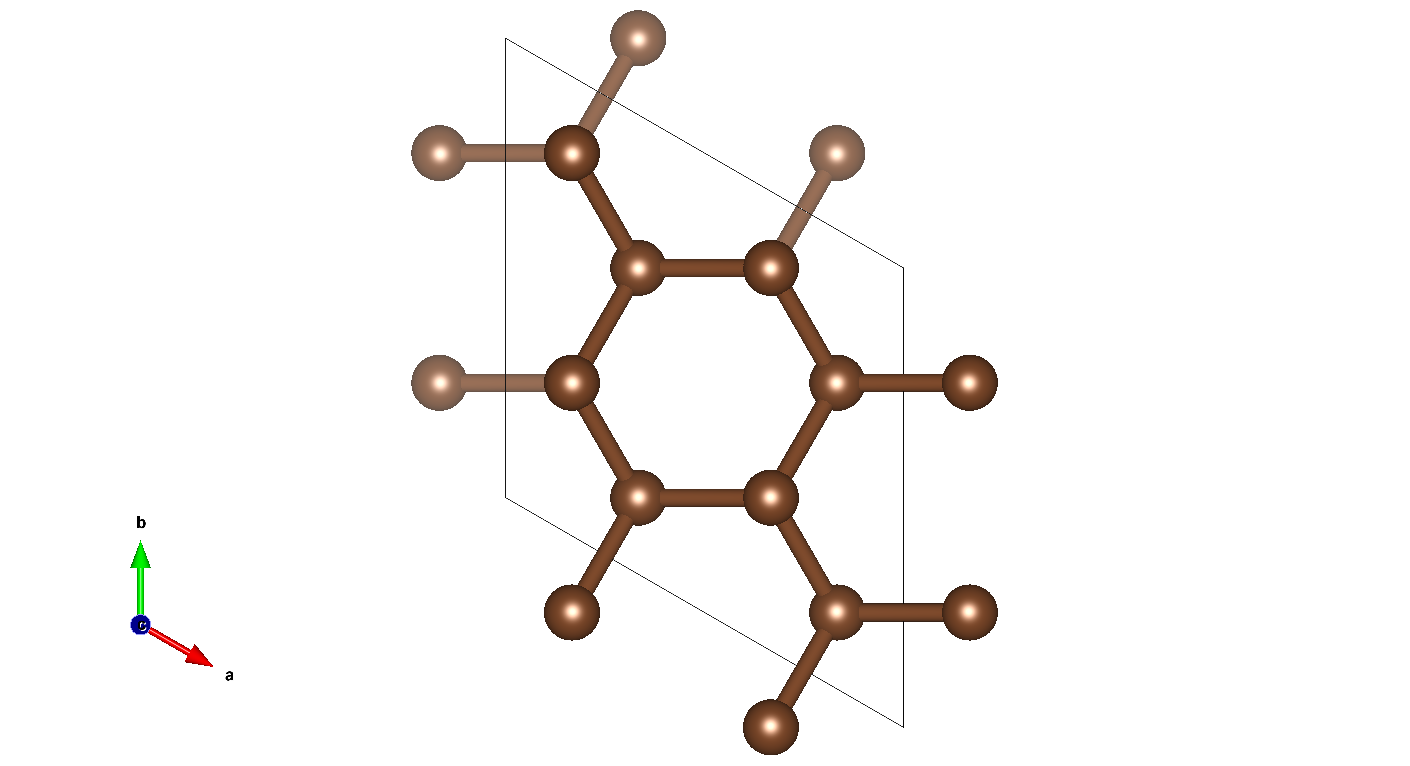
\includegraphics[width=0.5\textwidth, trim=0 0 30em 0,clip]{images/poscar_hex_16_hex-view.png}\\
    %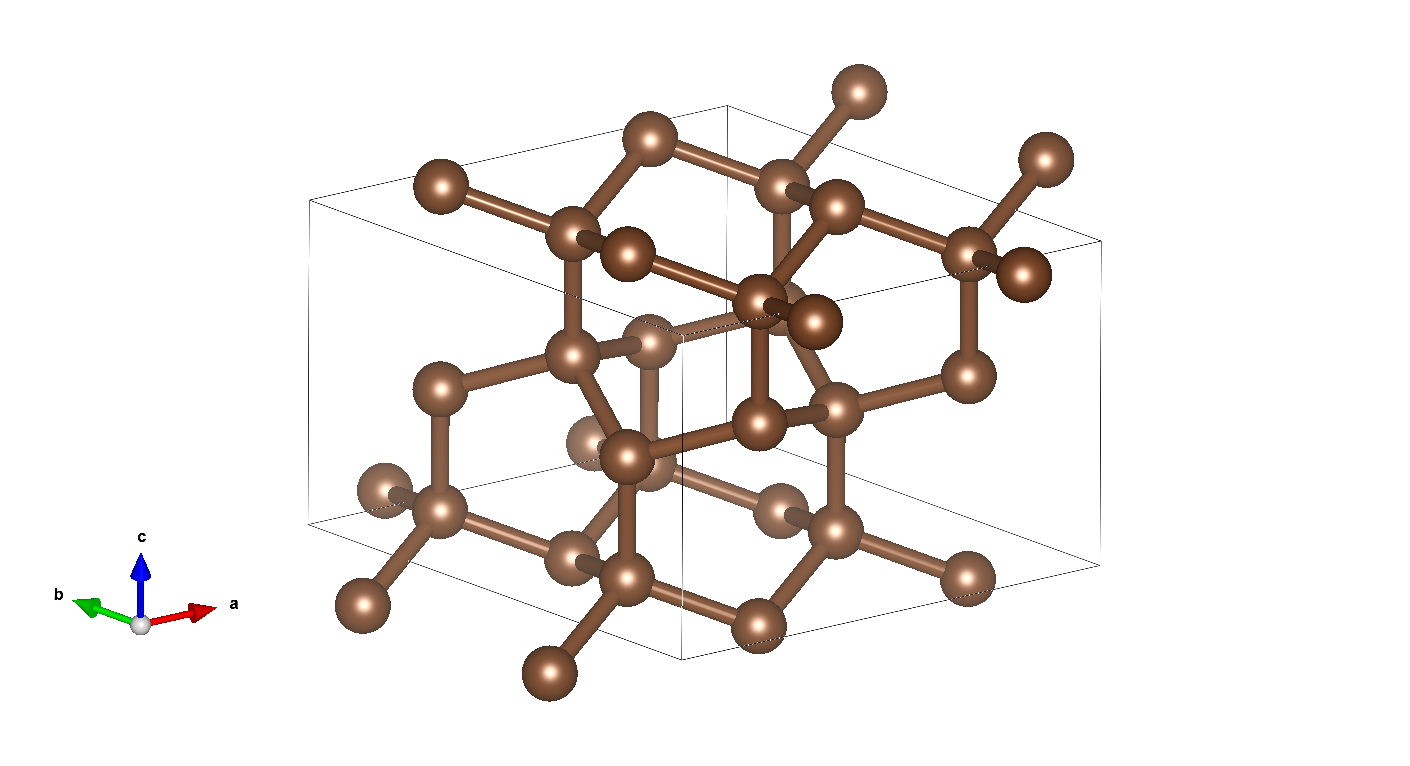
\includegraphics[width=0.5\textwidth, trim=0 0 27em 0,clip]{images/poscar_hex_16_birdseye.png}
  %\end{center}
%\end{frame}

\begin{frame}{Defect hexagonal diamond} %{{{1
  \begin{center}
    \begin{tabular}{cr}
      \raisebox{1cm}{Cubic diamond}   & 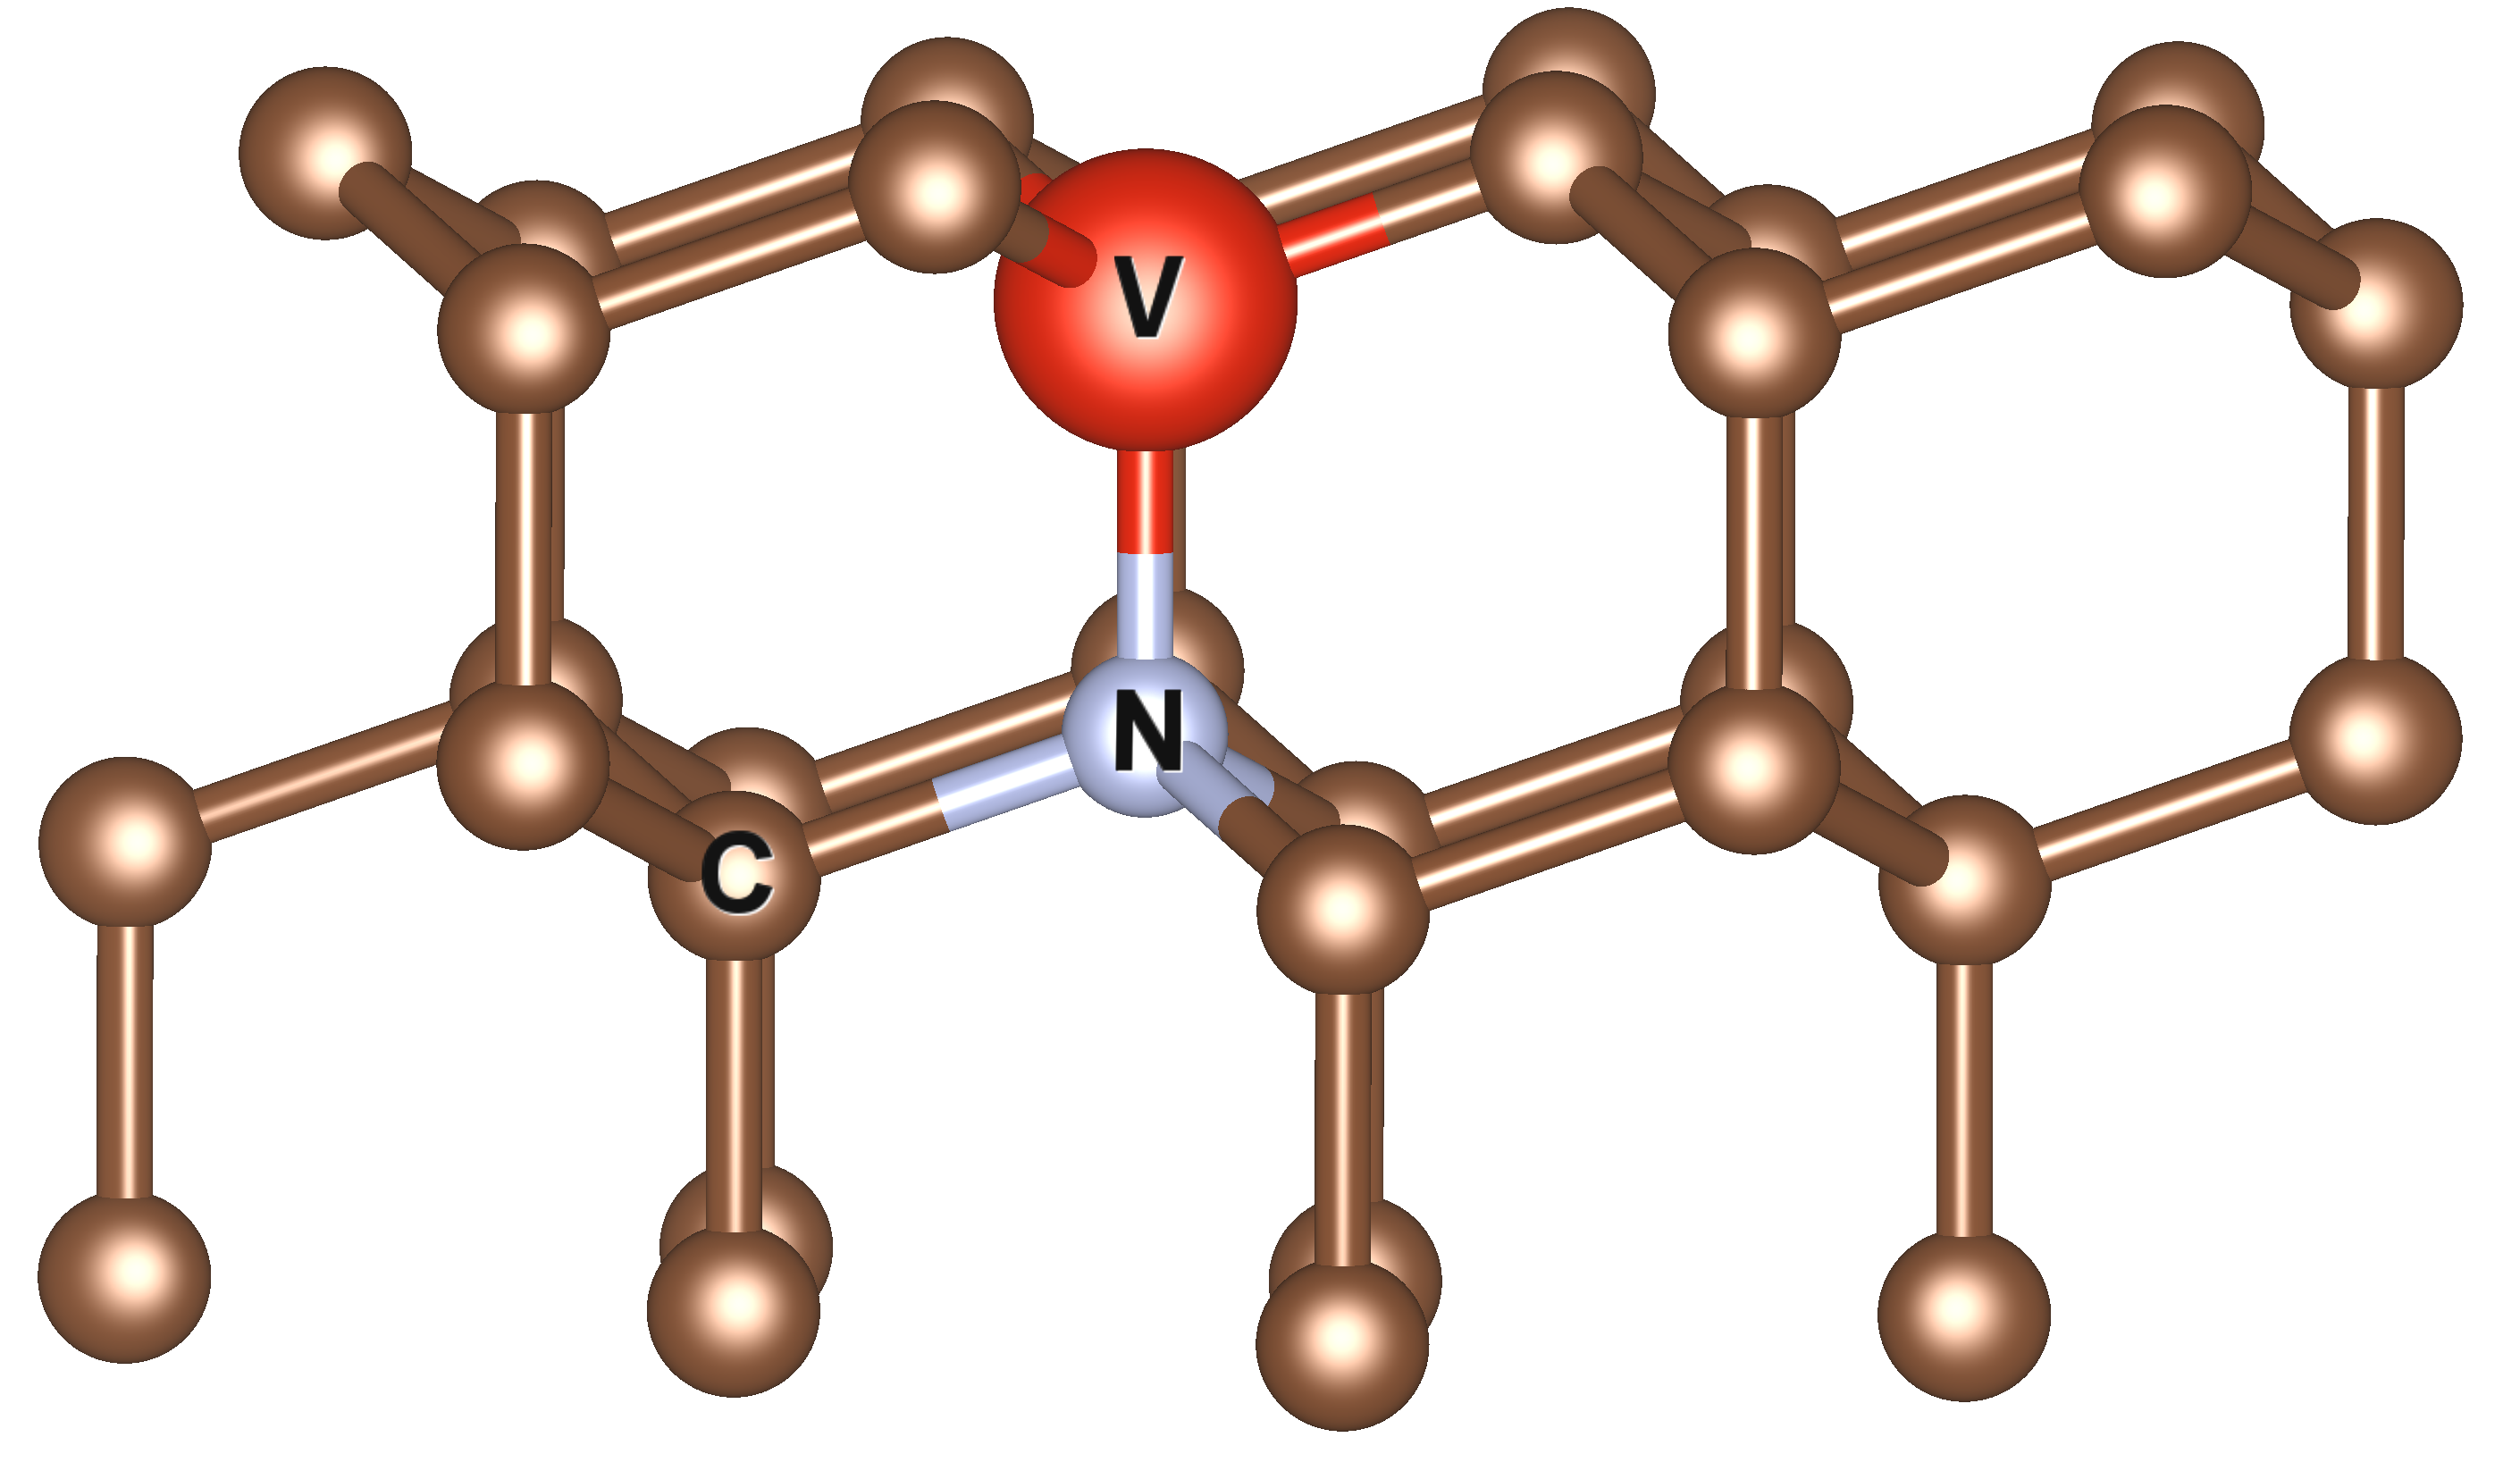
\includegraphics[width=0.4\textwidth]{images/POSCAR_16_view.png}\\
      \raisebox{1cm}{Hexagonal $ x $-type }
      &
      \only<1>{
        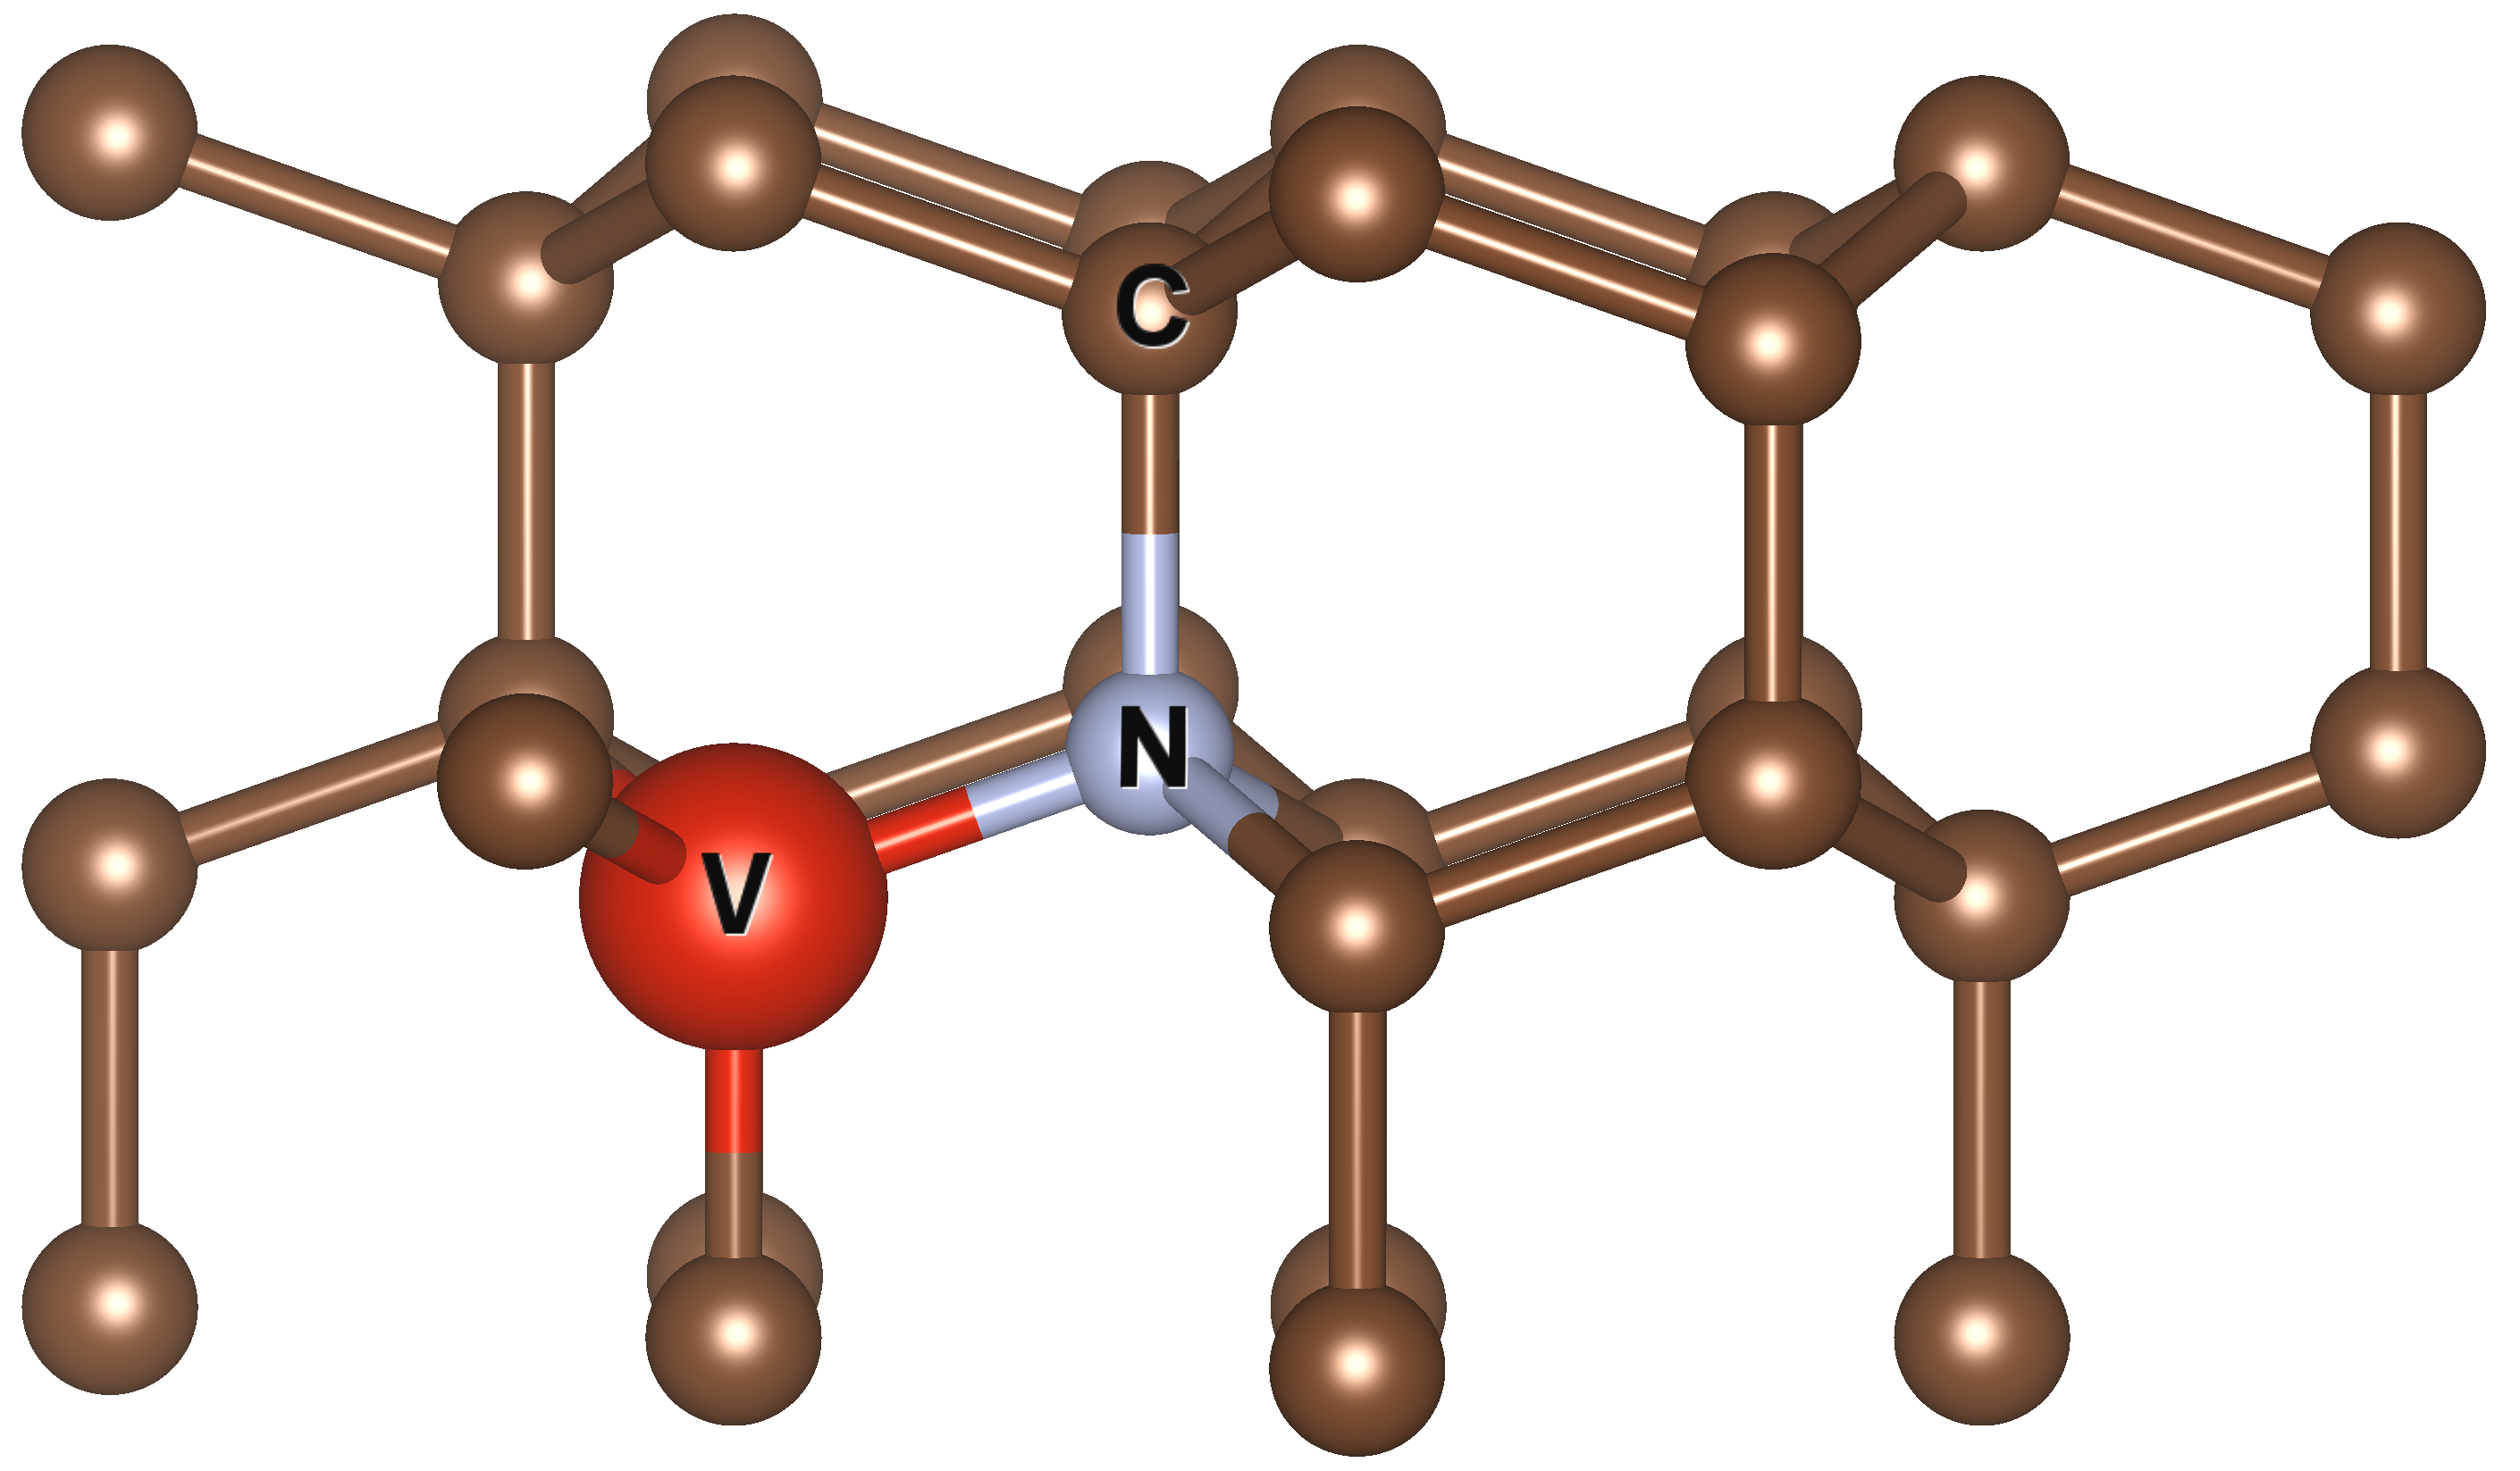
\includegraphics[width=0.4\textwidth]{images/POSCAR_16_x_view.png}
      }
      \only<2>{
        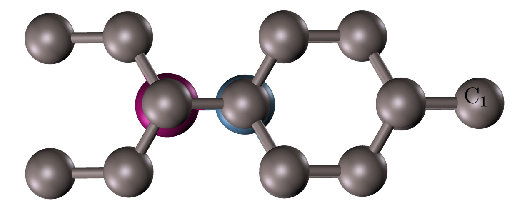
\includegraphics[width=0.4\textwidth]{images/hexagonal_view_above.pdf}
      }
      \\
      \raisebox{1cm}{Hexagonal $ z $-type } & 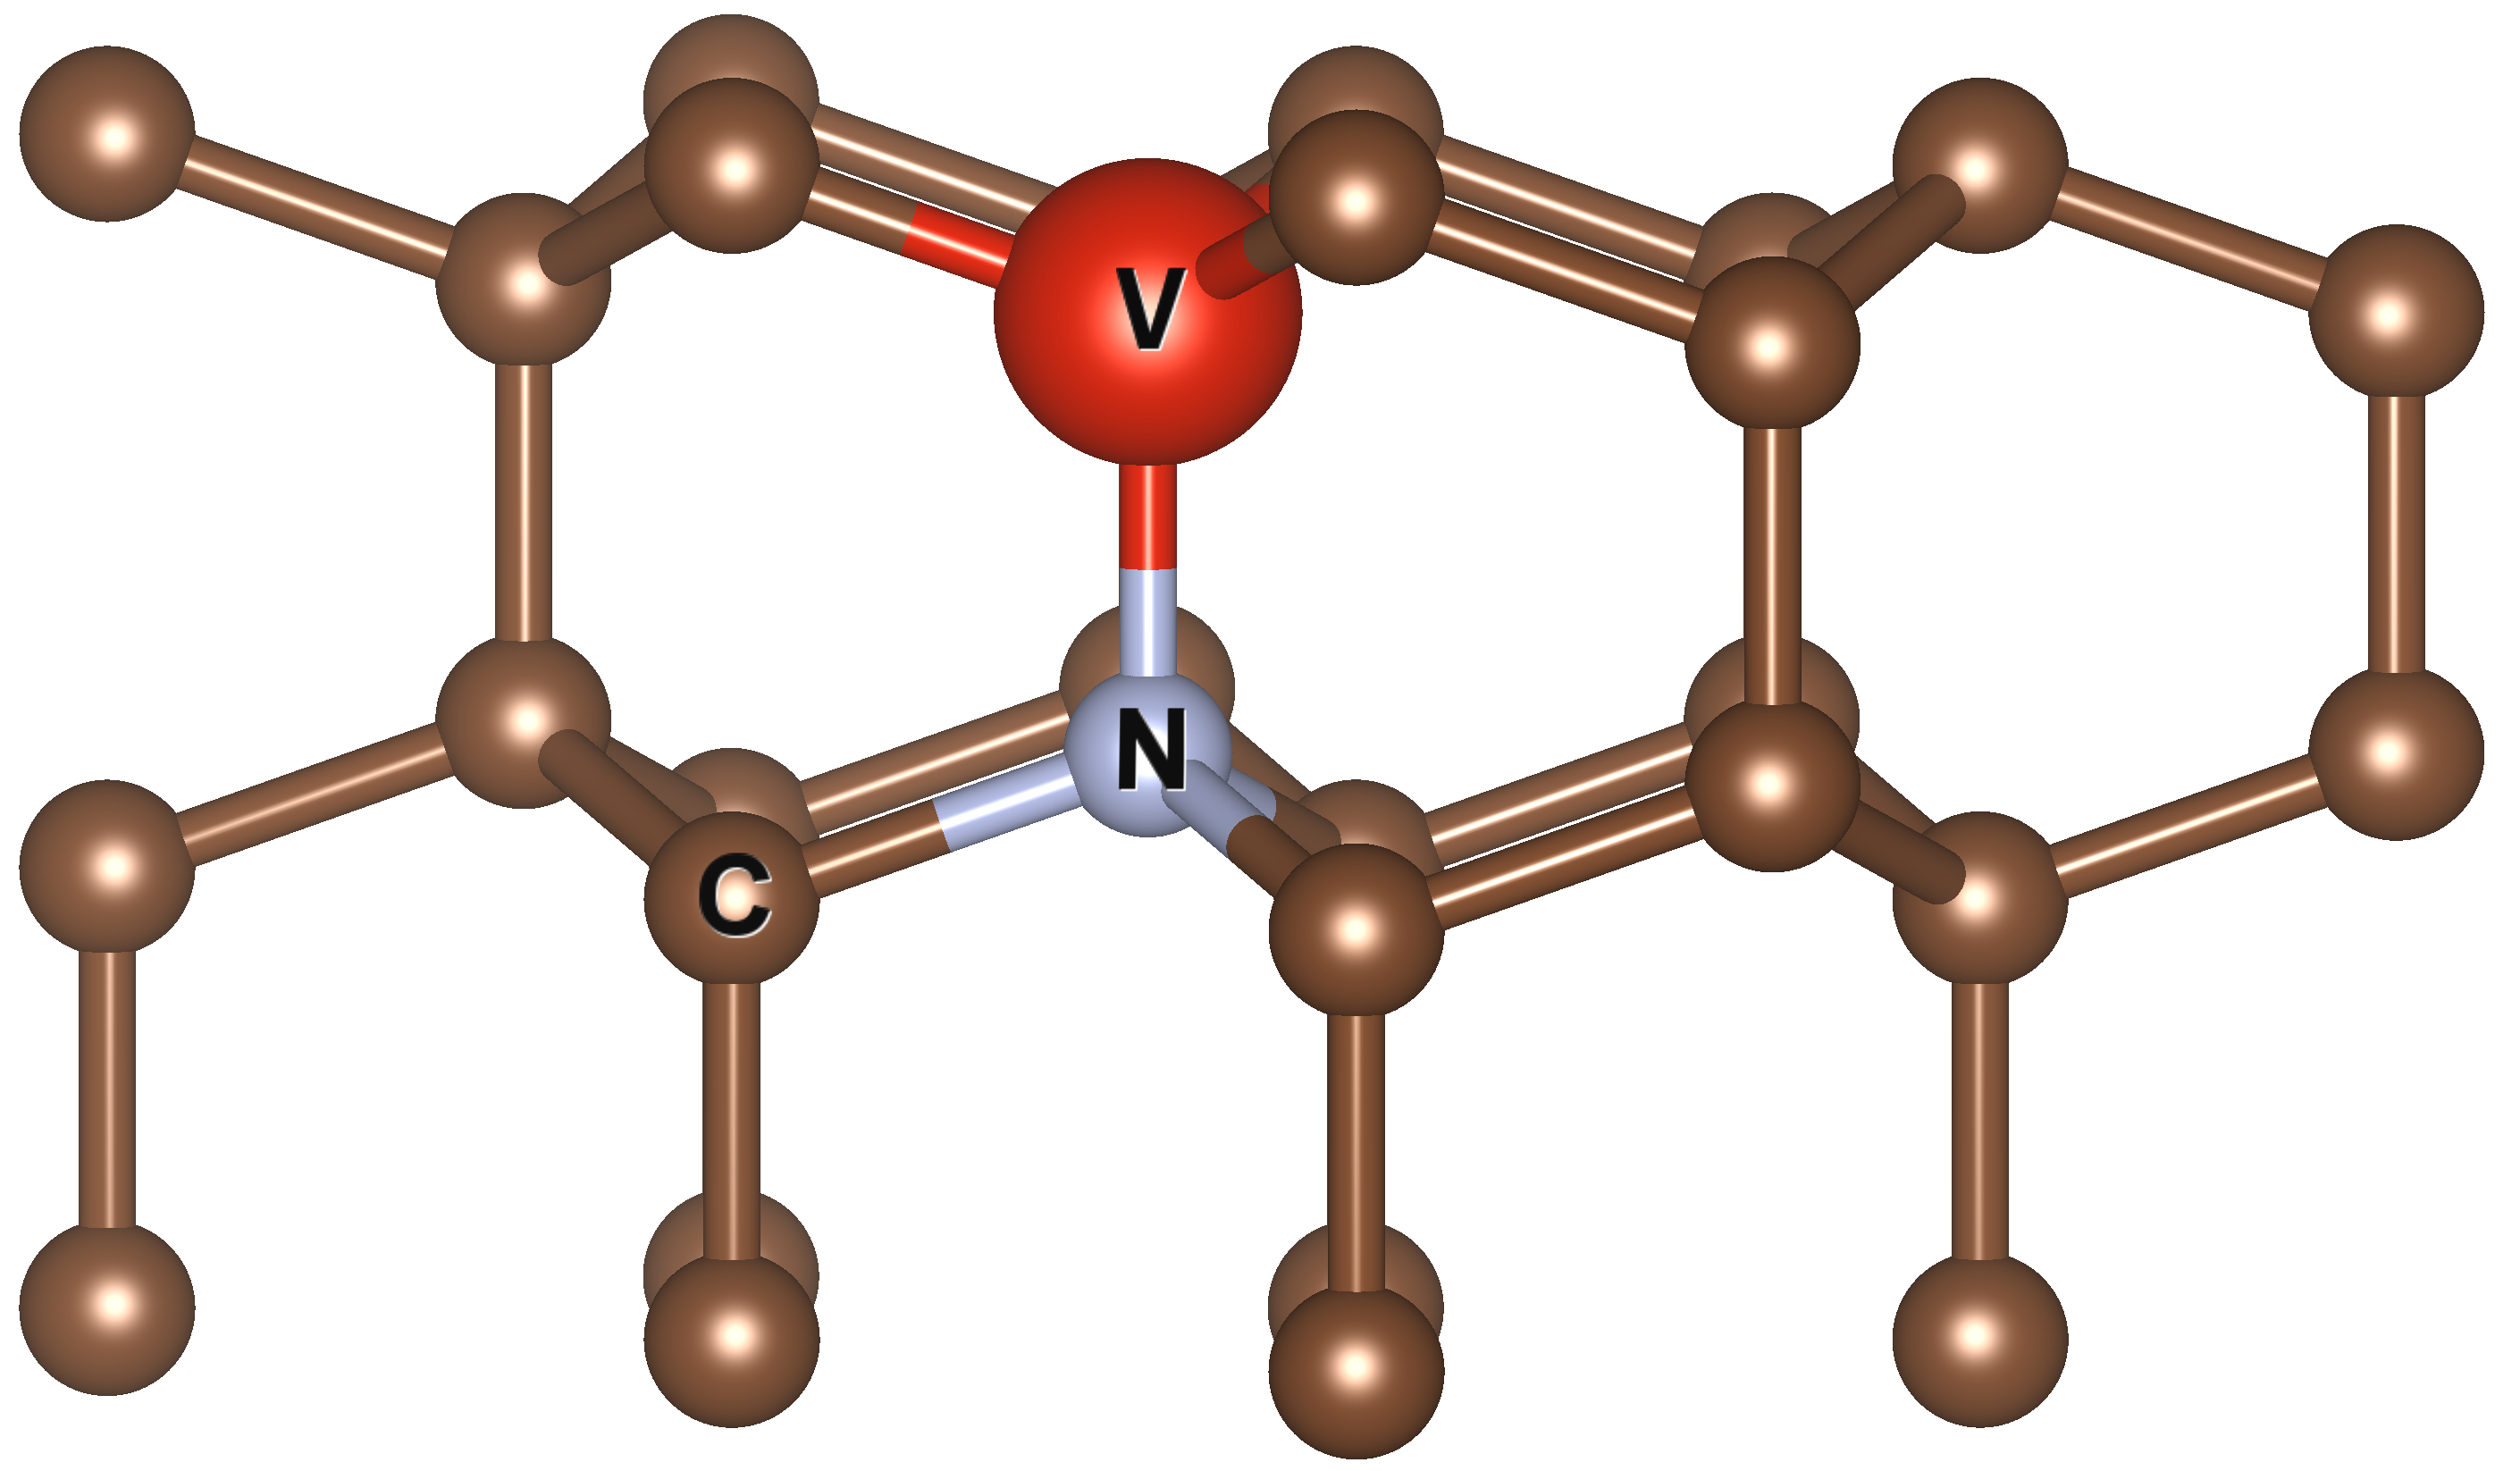
\includegraphics[width=0.4\textwidth]{images/POSCAR_16_z_view.png}
    \end{tabular}
  \end{center}
\end{frame}





\begin{frame}{DFT + DMRG}
  \includegraphics[width=\textwidth]{images/dmrg_algo_chart.pdf}
\end{frame}

%\section{Results} %{{{1
%\begin{frame}{ $ \mathsf{NV}^{-} $: Ground state $ ^3A_{2} $ } %{{{1
    \begin{tikzpicture}
      \node at (0,0) {
          \begin{columns}
            \begin{column}{0.3\textwidth}
              \includegraphics[height=1\textheight]{images/lumos/N_minus_cubic_128_dmatrix_encut_lumos.pdf}
            \end{column}
            \begin{column}{0.3\textwidth}
              \includegraphics[height=1\textheight]{images/lumos/N_minus_hexagonal_z_128_dmatrix_encut_lumos.pdf}
            \end{column}
            \begin{column}{0.3\textwidth}
              \includegraphics[height=1\textheight]{images/lumos/N_minus_hexagonal_x_128_dmatrix_encut_lumos.pdf}
            \end{column}
          \end{columns}
        };
      \node<2-> [fill,gray!10] at (0.23,1.5) {
        \includegraphics[height=0.4\textheight]{images/basic_level_definition_with_spin.pdf}
        };
      \end{tikzpicture}

\end{frame}



%\begin{frame}{ $ \mathsf{NV}^{-} $: Excited state $ ^3E $ } %{{{1
  \begin{center}
    \begin{columns}
      \begin{column}{0.3\textwidth}
        \includegraphics[height=1\textheight]{images/lumos/excited/N_minus_cubic_128_B_OUTCAR.pdf}
      \end{column}
      \begin{column}{0.3\textwidth}
        \includegraphics[height=1\textheight]{images/lumos/excited/N_minus_hexagonal_z_128_B_OUTCAR.pdf}
      \end{column}
      \begin{column}{0.3\textwidth}
        \includegraphics[height=1\textheight]{images/lumos/excited/N_minus_hexagonal_x_128_B_OUTCAR.pdf}
      \end{column}
    \end{columns}
  \end{center}
\end{frame}

%\begin{frame}{ $ \mathsf{NV}^{-} $: Vibronic scheme (PBE + 128 atomic cell)} %{{{1
  \begin{center}
    \includegraphics<1>[width=.5\textwidth]{images/vibronic.pdf}
  \end{center}
  \only<2>{
    \begin{columns}
      \begin{column}{0.3333\textwidth}
        \centering
        \textit{Cubic }
        \includegraphics[width=1\textwidth, trim=0 0 0em 0,clip]{images/abcd/abcd_128_zinc.pdf}
      \end{column}
      \begin{column}{0.3333\textwidth}
        \centering
        \textit{Hexagonal $ x $ }
        \includegraphics[width=1\textwidth, trim=0 0 0em 0,clip]{images/abcd/abcd_128_z.pdf}
      \end{column}
      \begin{column}{0.3333\textwidth}
        \centering
        \textit{Hexagonal $ z $ }
        \includegraphics[width=1\textwidth, trim=0 0 0em 0,clip]{images/abcd/abcd_128_x.pdf}
      \end{column}
    \end{columns}
  }
  \only<3->{
    \begin{columns}
      \begin{column}{0.3333\textwidth}
        \centering
        \textit{Cubic }
        \includegraphics[width=1\textwidth, trim=0 0 0em 0,clip]{images/abcd/abcd_128_zinc.pdf}
      \end{column}
      \begin{column}{0.3333\textwidth}
        \begin{center}
          \small
          \begin{tabular}{lc}
            \hline
            \multicolumn{2}{c}{Experimental data}\\
            \hline
            ZPL & 1.945\\
            \hline
            $ ^3A_2 \to ^3E^{*} $  & 2.180\\
            \hline
            $ S $  & 0.235\\
            \hline
            $  ^3E \to ^3A_2^{*} $ & 1.760\\
            \hline
            $ AS $  & 0.185\\
            \hline
          \end{tabular}
        \end{center}
      \end{column}
      \begin{column}{0.3333\textwidth}
        \begin{center}
          \small
          \begin{tabular}{lc}
            \hline
            \multicolumn{2}{c}{Calculations}\\
            \hline
            ZPL & 1.693\\
            \hline
            $ ^3A_2 \to ^3E^{*} $  & 1.842\\
            \hline
            $ S $  & 0.150\\
            \hline
            $  ^3E \to ^3A_2^{*} $  & 1.549\\
            \hline
            $ AS $  & 0.144\\
            \hline
          \end{tabular}
        \end{center}
      \end{column}
    \end{columns}
    }
  \end{frame}

%\begin{frame}{$ \mathsf{NV}^{-} $: ZFS } %{{{1
  \begin{itemize}
    \item
      \textit{Cubic diamond, convergence and comparison with the experimental result.}
  \end{itemize}
  \includegraphics[width=1.0\textwidth, trim=0 0 0em 0,clip]{images/zfs_cubic/plot_cubic.pdf}
\end{frame}

\begin{frame}{$ \mathsf{NV}^{-} $: ZFS cubic ($ \mathsf{NV}^{-}_{c} $), Hexagonal $ x,z $ ($ \mathsf{NV}_{x,z}^{-} $)   } %{{{1
  \includegraphics[width=1.0\textwidth, trim=0 0 0em 0,clip]{images/splitting_comparison/dmatrix_encut/N_all.pdf}
\end{frame}


%\begin{frame}{Expanding the defect:  } %{{{1
  \begin{center}
    \includegraphics[height=.9\textheight]{images/elements.pdf}
  \end{center}
\end{frame}

\begin{frame}{Expanding the defect} %{{{1
  \begin{center}
    \includegraphics[height=0.9\textheight]{images/elements_vacancies.pdf}
  \end{center}
\end{frame}


%\begin{frame}{ZFS map} %{{{1
  \begin{center}
    \includegraphics[width=1\textwidth]{images/splitting_comparison/dmatrix_encut/all.pdf}
  \end{center}
\end{frame}


%
\begin{frame}{Split vacancies: structural characterization} %{{{1
  \centering
  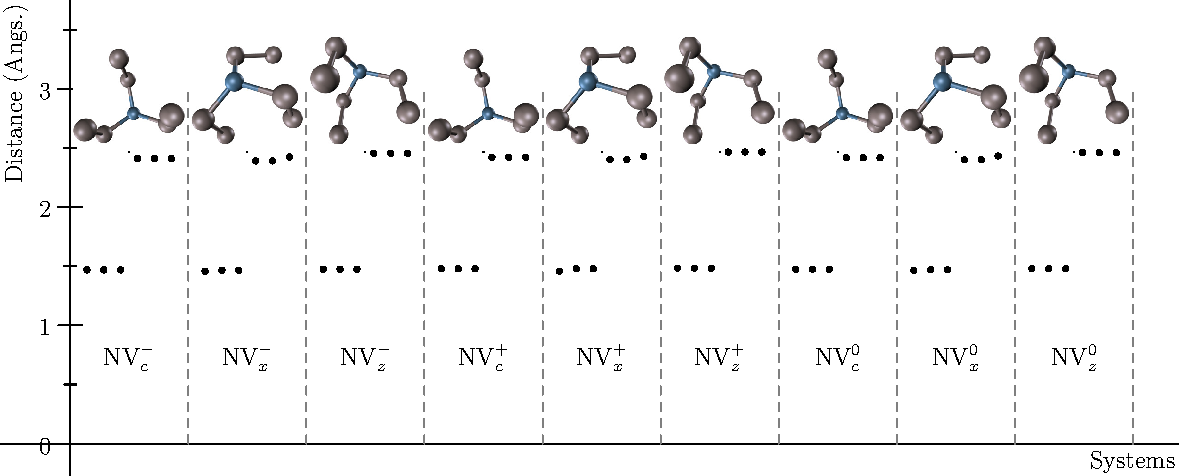
\includegraphics[height=.5\textheight]{images/split/split_N.pdf}\\
  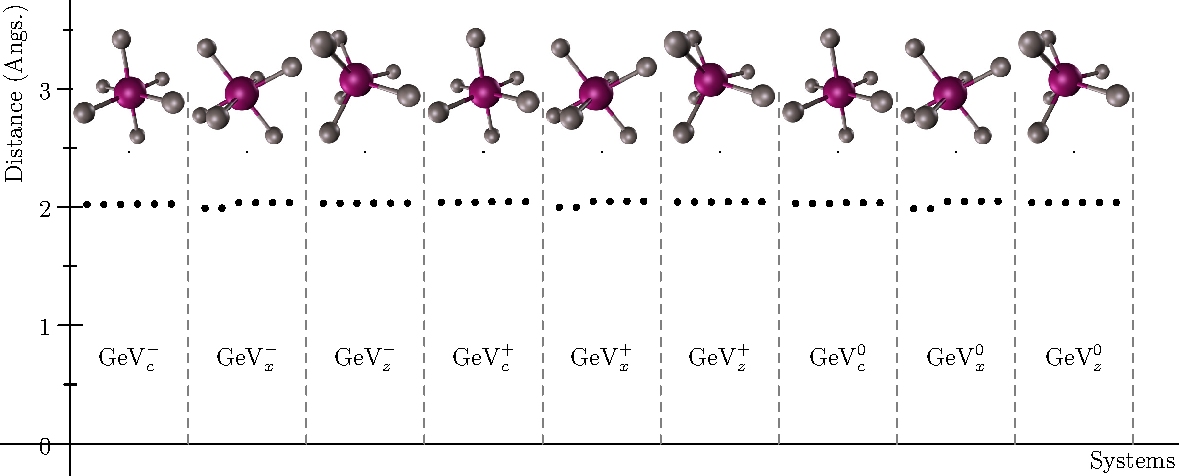
\includegraphics[height=.5\textheight]{images/split/split_Ge.pdf}
\end{frame}


%
\begin{frame}{Strain dependence of energy: $ \mathrm{NV}^{-} $ 216 cell} %{{{1
  \centering
  \begin{columns}
    \begin{column}{0.5\textwidth}
      \centering
      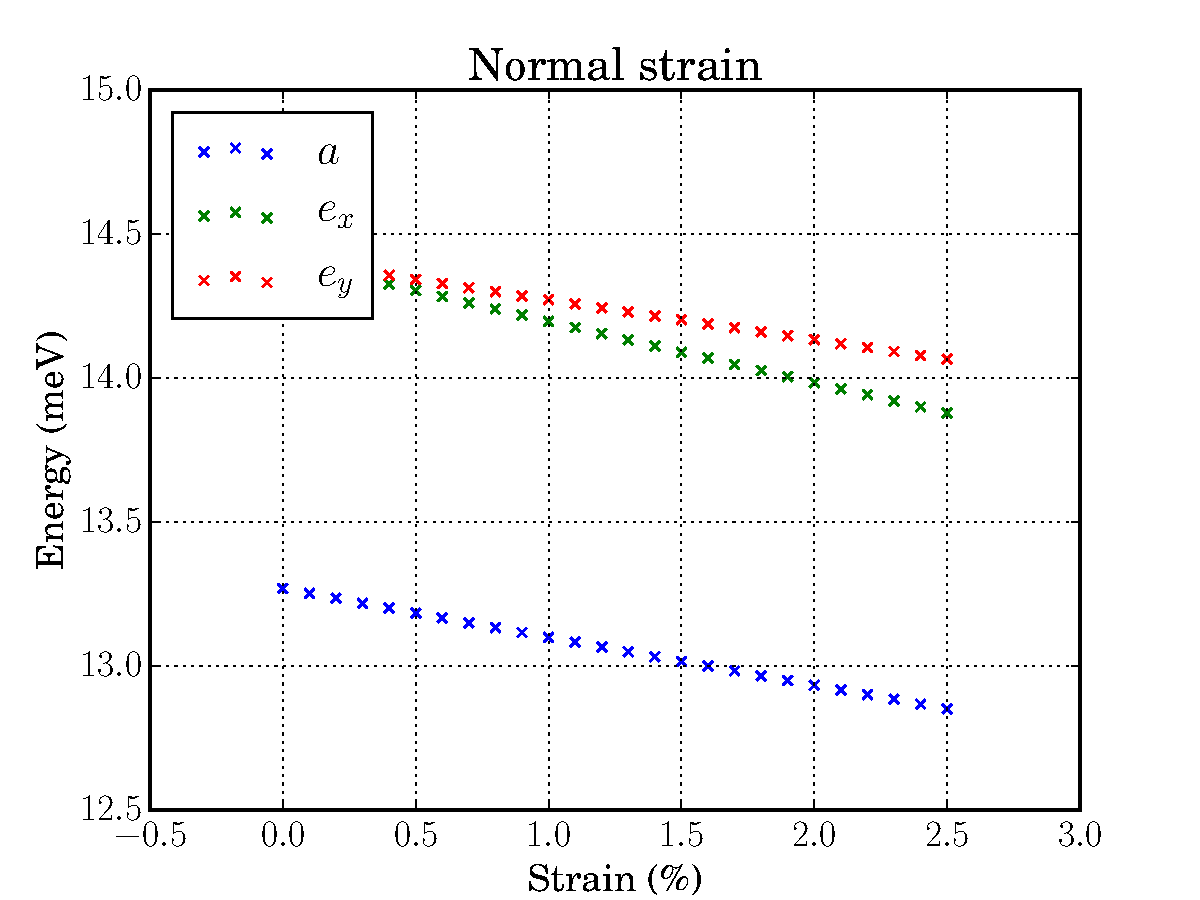
\includegraphics[width=1\textwidth]{images/strain/vasp-216-normal-relaxed.pdf}\\
      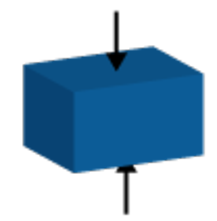
\includegraphics[width=0.2\textwidth]{images/strain/normal-strain.pdf}
    \end{column}
    \begin{column}{0.5\textwidth}
      \centering
      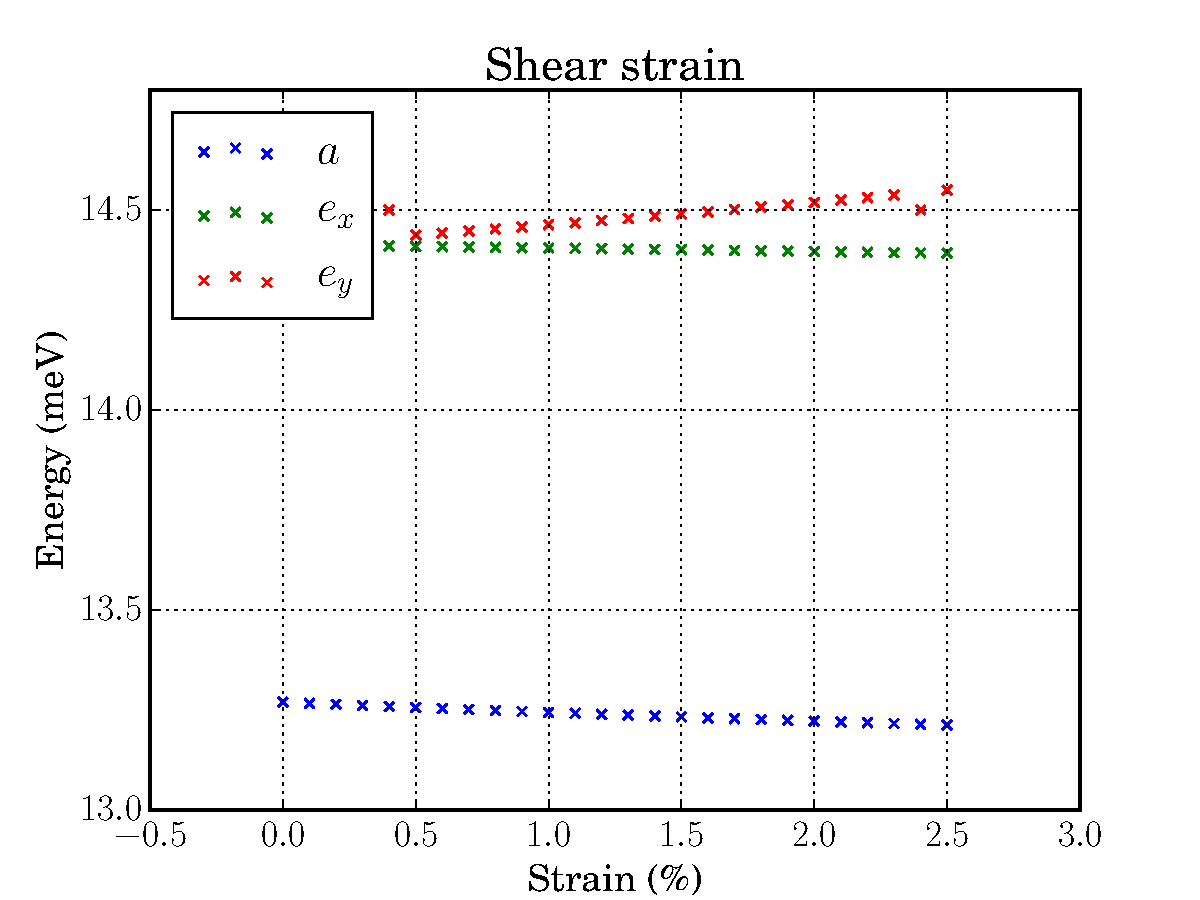
\includegraphics[width=1\textwidth]{images/strain/vasp-216-shear-relaxed.pdf}\\
      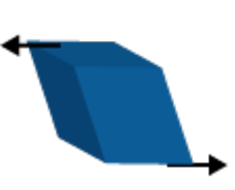
\includegraphics[width=0.2\textwidth]{images/strain/shear-strain.pdf}
    \end{column}
  \end{columns}
\end{frame}

\def\triplet{
  \raisebox{-3.4mm}{
    \boxed{
      \includegraphics[width=1cm]{images/dmrg/triplet.pdf}
    }
  }
}

\def\tripletTwo{
  \raisebox{-3.4mm}{
    \boxed{
      \includegraphics[width=1cm]{images/dmrg/triplet_2.pdf}
    }
  }
}


%\begin{frame}{DMRG\: Density Matrix Renormalization Group} %{{{1
  \centering
  \visible<1->{%
    \textbf{DFT}/\textbf{HF}
  }
  \visible<2->{%
    $ \quad \Rightarrow \quad $
    $ \triplet $
  }
  \visible<3->{%
    $ \quad \Rightarrow \quad $
    $ \ket{\Phi } =
     \ket \triplet $
  }
  \visible<4->{%
    \begin{center}
      Only one Slater determinant?
    \end{center}
  }
  \visible<5->{%
    $
      \ket{\Phi} =
      c_{1} \ket{\triplet} +
      c_{2} \ket{\tripletTwo} +
      \ldots?
    $
  }
  \visible<6->{%
    \begin{center}
      We may be missing part of the information \ldots
    \end{center}
  }
\end{frame}

\begin{frame}{DMRG\: Density Matrix Renormalization Group} %{{{1
  \centering
  %
  %
  \[
  \ket{\Phi} = \sum^{}_{I} c_{I} \ket{I}, \qquad \mbox{ $ I $ is a configuration}
  \]
  %
  %
  \visible<2->{%
    $ c_{I} $ explode with the number of orbitals.
  }
  \visible<3->{%
    Ansatz?
  }
  \visible<4->{%
    $$
    c_{I} =
    \sum^{}_{i_{1}, i_{2}, \ldots, i_{k-1}}
    \mathbf{M}^{n_{1}}_{i_{1}}
    \mathbf{M}^{n_{2}}_{i_{1}i_{2}}
    \mathbf{M}^{n_{3}}_{i_{2}i_{3}}
    \cdots
    \mathbf{M}^{n_{k-1}}_{i_{k-2}i_{k-1}}
    \mathbf{M}^{n_{k}}_{i_{k-1}}
    $$
  }
  \visible<4->{%
    $ \mathbf{M}_{ij} $ are matrices of dimension $ M $. $ k $ is the total number of orbitals and
    $ n_{k}(I) $ the occupation of the configuration $ I $ for the state $ k $.
  }
\end{frame}



\begin{frame}{DMRG: Results} %{{{1
  \begin{columns}
    \begin{column}{0.5\textwidth}
      \includegraphics[width=1.2\textwidth]{images/basic_levels.pdf}
    \end{column}
    \begin{column}{0.5\textwidth}
      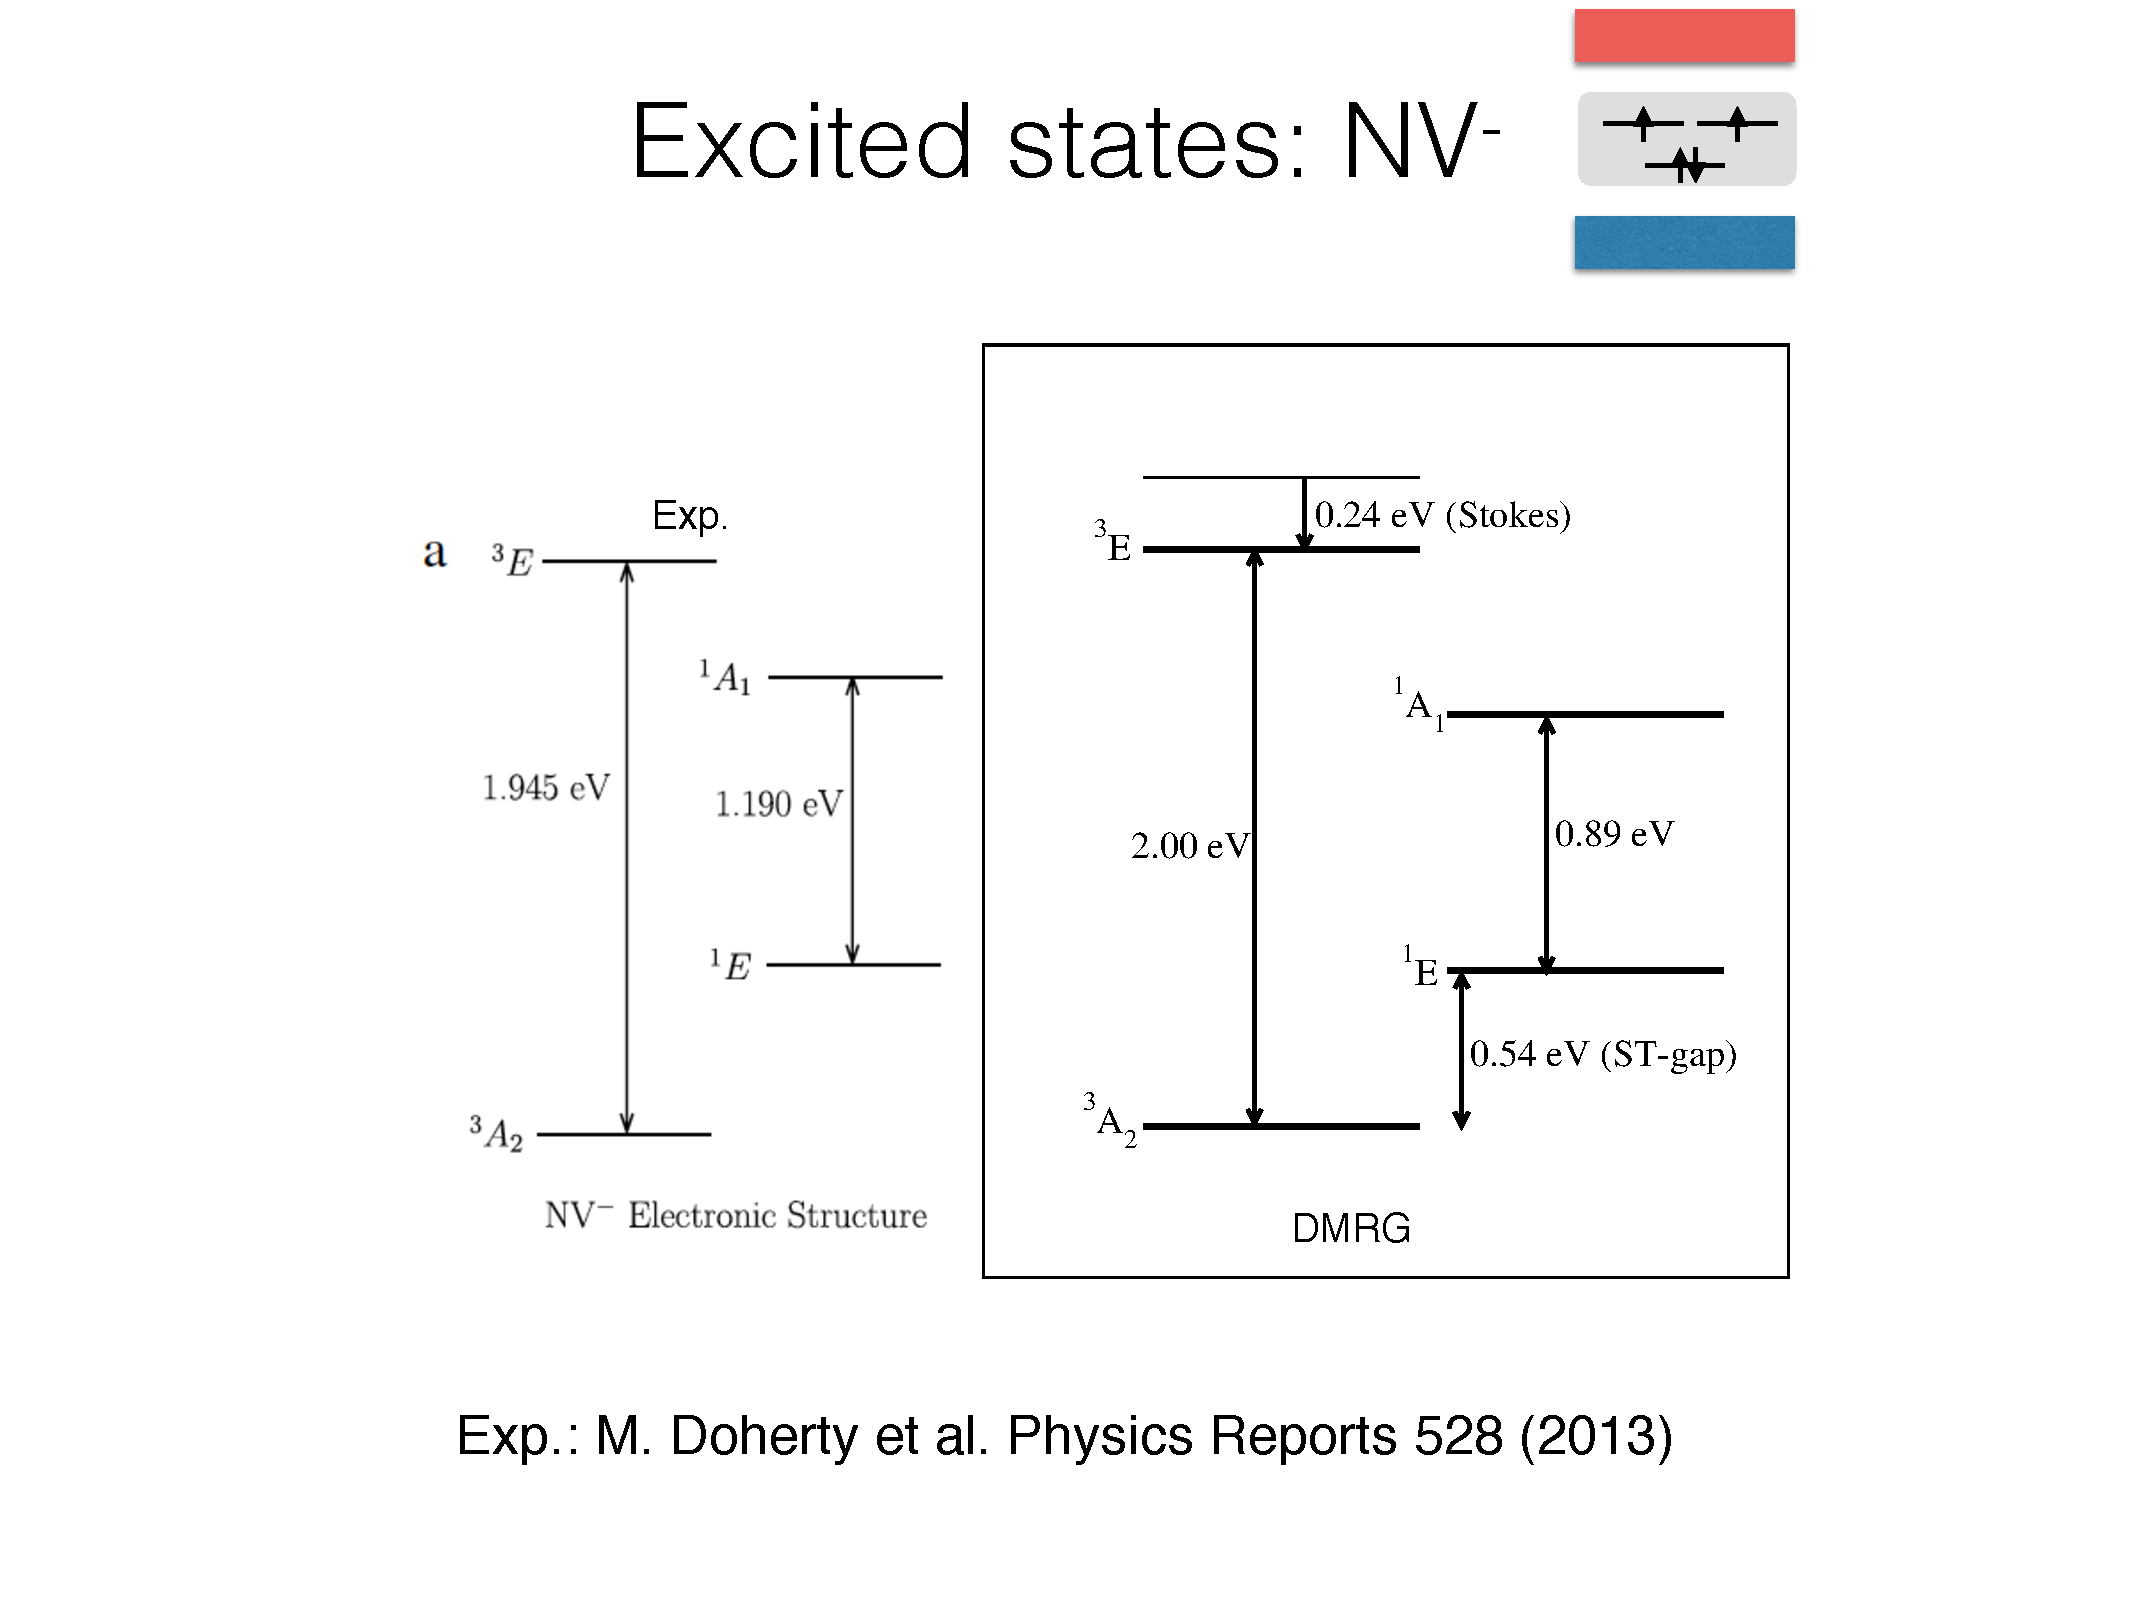
\includegraphics[width=1\textwidth, trim=500 200 190 200, clip]{images/dmrg_results.pdf}
    \end{column}
  \end{columns}
\end{frame}






%\section{Summary and outlook} %{{{1

\begin{frame}{Where we are, and where to go next\ldots} %{{{1
  \begin{itemize}
    \item
      Structural properties (split vacancies, bond lengths \ldots)
    \item
      ZPL (\textit{Zero Phonon Line}) calculation.
    \item
      ZFS (\textit{Zero Field Splitting}) tensor calculation.
    \item
      Strain dependence for ZFS tensor.
    \item
      Excited state calculations of the $ \mathrm{NV}^{-} $ centre with DMRG\@.
    \item
      \textbf{Beyond the Ground state:}\\
      \begin{itemize}
        \item
          DMRG for different $ \mathrm{XV} $ centres with interesting impurity
          atoms $ X $ (Ge, P, Si \ldots).
        \item
          \textit{Coupled Cluster} methods for solids to obtain a more
          \textit{robust} approach without any embedding approach.
      \end{itemize}
  \end{itemize}
\end{frame}

\begin{frame}{}
  
\includegraphics[width=.2\textwidth]{images/max_planck.png}\\
  \begin{columns}
    \begin{column}{0.5\textwidth}
      \textbf{Andreas Grüneis} group at the Max-Planck Institute for solid
      state research in Stuttgart, Germany.
    \end{column}
    \begin{column}{0.5\textwidth}
      \includegraphics[width=\textwidth]{images/group_photo.jpg}\\
      {\tiny
        A. Grüneis, K. Liao, T. Tsatsoulis, A. Gallo, T. Gruber, F. Hummel
      }
    \end{column}
  \end{columns}
  Acknowledgements:
  S. Sharma (Univ. Colorado Boulder), M. Doherty, P. Reddy, A. Alkauskas (ANU),
  H. Fedder (Swabian Instruments) and J.  Wrachtrup (Uni. Stuttgart)
\end{frame}

\plain{Thank you!}







\end{document}


% vim: spell fdm=marker :
